\chapter{Shearlets}

We want to be able to express efficiently Epipolar Plane Images, since this will reduce the number of minimum views needed to recover the light field of a scene; this task can be achieved by understanding the EPIs as signals and using signal processing machinery developed in the last twenty years, in this chapter we will explain in detail state-of-the-art methods on signal sparse-representation.

\bigskip

One can think a signal as a function (or something that can be represented as) that contains information about the behavior or attributes of some phenomenon \cite{Roland}, by this definition it actually could be a lot of things; it also depends the area you are working on, this definition will work or not. For example, in signal processing, arbitrary binary data streams are not considered as signals. For the sake of simplicity in this thesis we will agree to define a signal as a function that could represent video, image or audio and it will be either analog (evaluated with continuous parameters) or digital (evaluated with discrete parameters). 

\bigskip

In signal processing and applied harmonic analysis one can generally represent the signals in a space-time domain, but one cannot get always meaningful information in this representation; plenty of different signal transforms have been proposed along time, this transforms are obtained generally by finding basis of certain functional spaces (e.g. $L^2(\mathbb{R}^2)$) and present different features like sparse representation of signals that permits an efficient processing and storing of them. The most known signal transform for its effectiveness and tradition is the Fourier Transform, proposed by the French Mathematician Joseph Fourier, on his paper "Théorie analytique de la chaleur" in 1822 where he showed that some functiones could be written as an infinite sum of sines and cosines. 

\bigskip

If $f\in L^2(\mathbb{R}^n)$ then its Fourier transform $\hat{f}$ will be 
$$
\hat{f}(\xi) := \int_{\mathbb{R}^n}f(x)e^{-i\langle x,\xi\rangle}dx
$$

one can think of the coordinates $\xi$ of the Fourier space as frequencies of $f$, as one can see the Fourier transform $\hat{f}$ just gives information about the frequencies contained in $f$, but not at which time they occur; moreover, small changes in the neighborhood of some point $x\in\mathbb{R}^n$ could change significantly its Fourier transform, in general one would like a transform that is robust under this kind of changes. A direct solution for this issue is reflected in the short-time Fourier transform; whose mechanism is based in localization of the Fourier transform to a certain window of $f$ and then move the window through the whole domain. Let $g\in L^2(\mathbb{R})$ the window function, the short-time Fourier transform of $f\in L^2(\mathbb{R})$ associated with the window $g$ will be

$$
S_gf(t,\xi)=\int_{\mathbb{R}} f(x)\overline{g(x-t)}e^{-ix\xi}dx=\langle f,M_{\xi}T_tg\rangle = (\widehat{f\cdot T_t\overline{g}})(\xi)\text{,  } t,\xi\in\mathbb{R}
$$

where $T_t:L^2(\mathbb{R})\longrightarrow L^2(\mathbb{R})$ is the translation operator with parameter $t$, given by 
$$
T_tf(x)=f(x-t)
$$
and $M_{\xi}:L^2(\mathbb{R})\longrightarrow L^2(\mathbb{R})$ is the modulation operator, given by 
$$
M_{\xi} f(x)=e^{i\xi x}f(x)
$$

\bigskip 

One can associate to this transform the atoms $\{M_{\xi}T_tg\}_{(t,\xi)\in\mathbb{R}^2}$; for computational purposes one can discretize the transform by taking $(t,\xi)\in\Lambda=a\mathbb{Z}\times b\mathbb{Z}$ for some $a,b>0$; the resulting atoms $G(g,a,b):=\{g_{am,bn}=M_{bn}T_{am}\}_{(m,n)\in\mathbb{Z}}$, for some cases of $(a,b)\in\mathbb{R}$ $G(g,a,b)$ is a generating set of $L^2(\mathbb{R})$ with an explicit recovery formula and other features, such sequence of function are known as \textbf{frames} (in this particular case \textbf{Gabor frames}) and can be understand as the generalization of orthonormal bases, we will study them in detail on the Section~\ref{sec:ShearletsFrames}, for a further reading about Gabor frames one can check \cite{Gabor}.

\bigskip

We introduced Gabor frames to overcome some limitations of the Fourier transform; Gabor frames also present some limitations
\begin{itemize}
\item When the Gabor frame is also a orthonormal basis it doesn't have a good time-frequency localization \cite{Gabor}.
\item The size of the window $g$ does not change therefotherefotherefotherefotherefotherefotherefotherefotherefore Gabor frames are not sensible to very localized information, so for instance they will never detect a singularity or regularity information of a function.
\end{itemize} 
both limitations above can be overcome using \textbf{wavelets}.

\bigskip 

The concept of wavelets and the signal transform related was introduced first time 
in 1980s by the french mathematicians Morlet and Grossmann to refer to "small wave" (or \textit{ondelette} in french) when they were studying siesimic waves (check the original paper \cite{Grossman}). The \textit{continuous wavelet transform} of a function $f\in L^2(\mathbb{R})$ associated to a mother function $\psi\in L^2(\mathbb{R})$ is defined by 

$$
\begin{aligned}
\mathcal{W}_{\psi}f(a,b)&=\int_{\mathbb{R}}f(t)a^{-\frac{1}{2}}\overline{\psi\left(\frac{t-b}{a}\right)}dt\\
&=\langle f, T_bD_a\psi\rangle = (f\ast D_a\overline{\psi}^*)(b)\text{, } (a, b)\in\mathbb{R}^+\times\mathbb{R} 
\end{aligned}
$$

where $D_a:L^2(\mathbb{R}\longrightarrow L^2(\mathbb{R})$ is the dilation operator given by $D_a f(t)=a^{-\frac{1}{2}}f\left(\frac{t}{a}\right)$, and $f^*(t)=f(-t)$, $a$ is the scaling paramter (controls the size of the window) and $b$ is the translation parameter. If the mother function $\psi$ satisfy the admissibility condition 

$$
C_{\psi}:=\int_0^{\infty}\frac{|\hat{\psi}(\xi)|^2}{\xi}d\xi <\infty
$$

we will say that $\psi$ is a admissible wavelet. If one has an admissible wavelet, one can get an straightforward inversion or recovery formula as
$$
f=\frac{1}{C_{\psi}}\int_{\mathbb{R}}\int_0^{\infty} W_{\psi}f(a,b)T_bD_a\psi\frac{da}{a^2}db
$$

\bigskip

The sequence of wavelet atoms will be $\{\psi_{a,b}(t)=a^{-\frac{1}{2}}\overline{\psi\left(\frac{t-b}{a}\right)}\}_{(a,b)\in\mathbb{R}^+}$, so one can write the wavelet transform of $f$ as $W_{\psi}f(a,b)=\langle f,\psi_{a,b}\rangle$. One can discretize the wavelet transforms as by the inner product with the discrete set of wavelet atoms
$$
\psi_{j,m}(t):=a^{-\frac{1}{2}}\psi(a^{-j}t-bm)\text{,  } (j,m)\in\mathbb{Z}^2\text{,  } t\in \mathbb{R}\text{,   }(a,b)\in\mathbb{R}^+\times\mathbb{R}
$$

the set of discrete set of wavelet atoms is referred as wavelet system. Wavelets are very relevant in Signal Processing due their great features 
\begin{itemize}
\item One can get information about the regularity of a function $f$ by estimating bounds of its wavelet transform.
\item The scaling parameter permits us to detect very localized information, in particular is very effective detecting one dimensional singularities, this property leads to the construction of a Multiresolution Analysis (MRA) which is an important area in applied harmonic analysis(check \cite{Mallat} p. 264).
\item The unified treatment of both digital and continuous transforms permits an easy computational implementation.
\item It can represent sparsely one dimensional signals, in the sense that not a lot of coefficients will be significant so one can delete them and still get a good approximation of the original signal.
\end{itemize}

\bigskip

Over all the features that we just mentioned the one that gave most of its fame to the wavelet transform is the last one, i.e.\ sparse representation of one dimensional signals, for instance this porperty of wavelets is what the image compression standard JPEG 2000 is based on. It is worth it to study in more detail sparse representation of data.

\bigskip

It is not surprising that compression of data takes an important place in the academic research and industrial agenda nowadays. Our society generates and acquire a lot of data everyday that comes in a lot of different types and dimensions; the complexity of the processing of this raw data to extract some useful features in an understandable language grows with the dimensionality and size of the data. Even though, almost all data found in practical applications has the property that the relevant information which needs to be extracted or identified is sparse, that is, data are typically highly correlated and the essential information lives in lower dimensional subspaces (or manifolds). This information can be then captured using just few terms in an appropriate dictionary (e.g.\ some frame or orthonormal basis). 

\bigskip

The sparse representation property of data is important not only for data storage and transmission but also for feature extraction, classification, and other high-level tasks; finding a dictionary which sparsely represents a certain data class involves deep understanding of its dominant properties, which are typically associated with their geometric properties; for a deep treatment of this one can read \cite{IntroShearlets} and \cite{Gitta-Lim}.

\bigskip

So far we have just mentioned the sparse representation property for one-dimensional signals and also the existence of straight forward and fast algorithmic implementations; the latter is based in the general machinery to construct orthonormal wavelet bases known as \textit{Multiresolution Analysis} (MRA). In the one dimensional case, this is defined as a sequence of closed subspaces $(V_j)_{j\in\mathbb{Z}}$ of $L^2(\mathbb{R})$ known as the scaling spaces which satisfies the following properties

\begin{enumerate}
\item[(a)] $\{0\}\subseteq\ldots\subset V_{-2}\subset V_{-1}\subset V_0\subset V_1\subset V_2\subset\ldots L^2(\mathbb{R})$.
\item[(b)] $\cap_{j\in\mathbb{Z}}V_j=\{0\}$ and $\overline{\cup_{j\in\mathbb{Z}}V_j}=L^2(\mathbb{R})$.
\item[(c)] $f\in V_j$ if and only if $D_2^{-1}f\in V_{j+1}$.
\item[(d)] There exists a $\varphi\in L^2(\mathbb{R})$, called \textit{scaling function}, such that $\{T_m\varphi:m\in\mathbb{Z}\}$ is an orthonormal basis for $V_0$.
\end{enumerate}

This enables the decomposition of functions into different "resolution" levels associated with the so called wavelet spaces $W_j$, $j\in\mathbb{Z}$ which are defined by considering the orthogonal complements
$$
W_j:= V_{j+1}\ominus V_j\text{,  } j\in\mathbb{Z}
$$

This Multiresolution Analysis let us not only to decompose $L^2(\mathbb{R})$ as a direct sum of wavelet spaces but also gives us an alternative orthonormal basis with both the wavelet and the scaling fuction, of the form

$$
\{\varphi_m=T_m\varphi=\varphi(\cdot-m):m\in\mathbb{Z}\}\cup\{\psi_{j,m}:j\geq 0,m\in\mathbb{Z}\}
$$

where the scaling function take care of the low-frequency region $V_0$ and the wavelet terms of the complementary space $L^2(\mathbb{R})\ominus V_0$. One can read \cite{Mallat}. 

\bigskip

In this thesis we are interested in image processing, if one would like to apply wavelets to imaging science an extension of the theory to $L^2(\mathbb{R}^2)$ is necessary. For a painless extension we can introduce the concept of tensor products of Hilbert spaces. If $\mathcal{H}_1$ and $\mathcal{H}_2$ are two Hilbert spaces the tensor product is a bilinear operator $\otimes:\mathcal{H}_1\times\mathcal{H}_2\longrightarrow \mathcal{H}_1\otimes\mathcal{H}_2$ where $\mathcal{H}_1\otimes\mathcal{H}_2$ is a new Hilbert space.

\bigskip

We can use strongly the fact that the tensor product of orthonormal bases is an orthonormal basis of $\mathcal{H}_1\otimes\mathcal{H}_2$. In the case of $\mathcal{H}_1=\mathcal{H}_2=L^2(\mathbb{R})$ and $f,g\in L^2(\mathcal{R})$, then $f\otimes g\in L^2(\mathbb{R}^2)$ is given by

$$
(f\otimes g)(x_1,x_2)=f(x_1)g(x_2)\text{,  } (x_1,x_2)\in\mathbb{R}^2,
$$

and $\mathcal{H}_1\otimes\mathcal{H}_2=L^2(\mathbb{R}^2)$. This concepts leads to the next theorem.

\bigskip

\begin{thm}[Two-dimensional wavelets]
Let $(V_j)_{j\in\mathbb{Z}}$ be an MRA for $L^2(\mathbb{R})$ with scaling function $\varphi\in L^2(\mathbb{R})$ and associated wavelet $\psi\in L^2(\mathbb{R})$. For $(x_1,x_2)\in\mathbb{R}^2$, we define
$$
\begin{aligned}
&\psi^1(x_1,x_2):=\varphi(x_1)\psi(x_2),\\
&\psi^2(x_1,x_2):=\psi(x_1)\varphi(x_2),\\
&\psi^3(x_1,x_2):=\psi(x_1)\psi_(x_2)
\end{aligned}
$$
Then 
$$
\{\psi_{j,m}^k(x_1,x_2)=2^{-j}\psi^k(2^{-j}x_1-m_1,2^{-j}x_2-m_2)\text{: } m=(m_1,m_2)\in\mathbb{Z}^2,k=1,2,3\}
$$
is an orthonormal basis for the wavelet space $W^2_j$, given by $V^2_j\oplus W^2_j=V^2_{j-1}$. Moreover,
$$
\{\psi_{j,m}^k\text{:  }j\in\mathbb{Z},m=(m_1,m_2)\in\mathbb{Z}^2,k=1,2,3\}
$$
is an orthonormal basis for $L^2(\mathbb{R}^2)$.
\end{thm}
\begin{proof}
One can find the proof on \cite{Mallat}, pp. 340-346.
\end{proof}

\bigskip

There exists more general non-separable two dimensional wavelets transforms using the continuous affine group to generalize the dilation operator $D_a$ to $D_M$ for two-dimensional invertible matrices $M$. The traditional theory of wavelets is based on the use of isotropic dilations and therefore is esentially a one-dimensional theory, so it is unable to give additional information about the geometry of the set of singularities of a function or distribution that are multivariate. The main problem is that the isotropic wavelet transform is simple but lacks of directional sensitivity and the ability to detect the multidimensional geometry of a function or distribution $f$.

\bigskip

One can formalize the notion of approximation quality using the concept of best $N$-term approximation. We will provide the general definition applied to dictionaries (collection of vectors on a Hilbert space $\{\varphi_i: i\in I\}\subseteq \mathcal{H}$ with $I$ finite or countable infinite).

\bigskip

\begin{defn}[Best N-term Approximation]
Let $D:=\{\varphi_i\text{:  }i\in I\}\subseteq \mathcal{H}$ be a dictionary. Consider a vector $x\in\mathcal{H}$ and an integer $N\in\mathbb{N}$. Then the \textit{best N-term approximation of x} with respect to $D$ is defined by the solution of the following minimization problem:
$$
\min_{I_N,(c_i)_{i\in I_N}}||x-\sum_{i\in I_N} c_i\varphi_i|| \text{ subject to } I:N\subseteq I,\# I_N\leq N
$$
\end{defn}

\bigskip

The best N-term approximation $f_N$ of $f\in L^2(\mathbb{R}^2)$ with respect to the dictionary formed by the wavelet basis can be understand as the obtained by approximating $f$ from its $N$ largest wavelet coefficients in magnitude. Let $\Lambda_N$ the index set corresponding to the $N$- largest wavelet coefficients $|\langle f,\psi_{\lambda}\rangle|$ associated with some wavelet basis $(\psi)_{\lambda\in\Lambda}$, the best $N$-term approximation will be
$$
f_N=\sum_{\lambda\in\Lambda_N}\langle f,\psi_{\lambda}\rangle\psi_{\lambda}
$$

\bigskip

To study the approximation of natural images by the wavelets, we first need to introduce a definition of what we will understand mathematically as a natural image, the so called \textit{cartoon-like functions}.

\bigskip

\begin{defn}[Cartoon-like functions]
The class of \textit{cartoon-like functions} $\mathcal{E}^2(\mathbb{R}^2)$ is defined as the set of functions $f:\mathbb{R}^2\longrightarrow \mathbb{C}$ of the form $f= f_0+\chi_B f_1$. Here, we assume that $B\subseteq [0,1]^2$ where $\partial B\in C^2$ and bounded curvature. Moreover, $f_i\in C^2(\mathbb{R}^2)$ with $||f_i||_{C^2}\leq 1$ and $\text{supp} f_i\subset [0,1]^2$ for $i=0,1$. 
\end{defn}

\bigskip

\begin{figure}[h!]
\centering
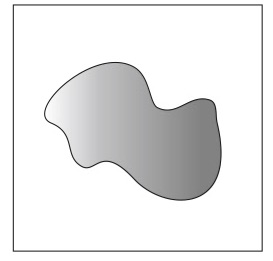
\includegraphics[width = 0.4 \textwidth]{./Diagrams/cartoon-like.jpg}
\caption{Example of a cartoon-like image. Figure taken from \cite{IntroShearlets} pp. 9}
\label{fig:cartoon-like}
\end{figure}

Now, let $f$ be a cartoon-like image containing a singularity along a smooth curve and $\{\psi_{j,m}\}$ be a standard wavelet basis of $L^2(\mathbb{R}^2)$. For $j$ sufficiently large, the only significant wavelet coefficients $\langle f,\psi_{ j,m}\rangle$ are the ones associated with the singularity. At each scale $2^{-j}$, each wavelet $\psi_{j,m}$ is supported inside a box of size $2^{-j}\times 2^{-j}$, there exist about $2^j$ elements of the wavelet basis overlapping the singularity curve. The associated wavelet coefficients are controlled by 

$$
|\langle f,	\psi_{j,m}\rangle|\leq ||f||_{\infty}||\psi_{j,m}||_{L^1(\mathbb{R}^2)}\lesssim 2^{-j}
$$

It follows that the $N$-th largest wavelet coefficient in magnitude, denoted by $\langle f,\psi_{j,m}\rangle_{(N)}$, is bounded by O($N^{-1}$) (since $N\leq 2^j$). Thus, if $f$ is approximated by its best $N$-term approximation $f_N$, the $L^2$ error (called  best $N$-term approximation error) obeys

$$
\sigma_N(f,\{\psi_{j,m}\}_{j,m})^2=||f-f_N||^2_{L^2(\mathbb{R}^2)}\leq \sum_{\ell\geq N}|\langle f,\psi_{j,m}\rangle_{(l)}|^2\lesssim N^{-1}
$$

This estimate is actually tight, in the sense that there exist cartoon-like images for which the best $N$-term approximation error is

$$
\sigma_N(f,\{\psi_{j,m}\}_{j,m})\approx N^{-\frac{1}{2}}
$$
the proof of this result can be founded in \cite{Mallat}.

Even this looks like a nice result, it is far from optimal.

\bigskip

\begin{thm}
\label{C3S2T1}
Let $\{\psi_{\lambda}\}_{\lambda\in\Lambda}\subseteq L^2(\mathbb{R}^2)$ be a frame for $L^2(\mathbb{R}^2)$. Then the optimal best $N$-term approximation error for any $f\in\mathcal{E}^2(\mathbb{R}^2)$ is
$$
\sigma_N(f,\{\psi_{\lambda}\}_{\lambda\in\Lambda})=O(N^{-1})
$$
\end{thm}
\begin{proof}
In Section~\ref{sec:ShearletsFrames} we will define the concept of frame. This result was proved by Donoho in 2001 on \cite{DonohobestNterm}, so one can refer to his proof.
\end{proof}

\bigskip

As we mentioned before, the problem with wavelets that does not make them to approach efficiently multivariate data is related to its isotropic scaling characteristic that makes them not sensible to directions. The question that can arise is, "Why should we care about anisotropic features related to multidimensional singularities?"; all the multivariate data are typically dominated by anisotropic features such as singularities on lower dimensional embedded manifolds; for example by edges in natural images or shock fronts in the solutions of transport equations. 

\begin{figure}[h!]
\centering
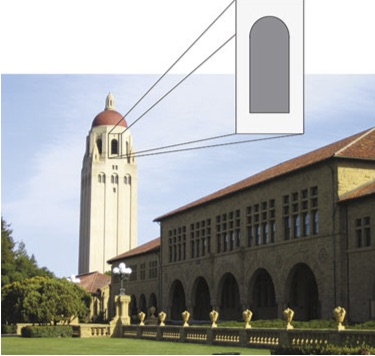
\includegraphics[width = 0.7\textwidth]{./Diagrams/edges-images.jpg}
\caption{Natural images governed by anisotropic structures. Figure taken from \cite{IntroShearlets} pp. 8}
\label{edges-images}
\end{figure}

\bigskip

The bound result of theorem~\ref{C3S2T1} works as a benchmark for optimally sparse approximation of two-dimensional data in form of cartoon-like functions. Moreover, to proof theorem~\ref{C3S2T1} Donoho used adapted triangulations, which suggests that analyzing elements with elongated and orientable supports are required to get optimally sparse approximations of piecewise smooth two-dimensional functions. This observation leaded to two different approaches for solving this problem, the curvelets (proposed by E. Candès and D. Donoho in 1999 \cite{Curvelets}), and the shearlets (proposed by Kanghui Guro, Gitta Kutyniok and Demetrio Labate in 2005 \cite{FirstShearlets}), both are able to achieve the same optimal approximation rate; the one used in this thesis to sparsely represent EPIs is the latter due the possibility to develope a faithful implementation. 

\section{Shearlet Systems and Transform}
\label{sec:shearletsystem}

We just discussed the limitations of wavelet systems in higher dimensions, we will then the concept of shearlet systems as a framework to solve these limitations. We also mentioned that in order to achieve optimally sparse approximations of signals with anisotropic singularities such as cartoon-like images, the analyzing elements must be made by waveforms ranging over several scales, orientations, and locations with the ability to become very elongated. One need then the combination of an appropriate scaling operator to generate elements at different scales, an orthogonal operator to change their orientations, and a translation operator to displace the elements over the two-dimensional plane. 

\bigskip

By tradition and effectivenes one can use the family of dilation operators $D_{A_a}$, $a>0$ based on parabolic scaling matrices $A_a$ of the form

\begin{equation}
\label{eq:scaling}
A_a:=
\left(
\begin{matrix}
a & 0 \\
0 & a^{1/2}
\end{matrix}
\right)
\end{equation}

This is the first approach to a scaling operator by the long history of parabolic scaling in harmonic analysis literature \cite{Fefferman}; the so called \textit{Classical Shearlets} use this approach, one can generalize the scaling using matrices of the form 

\begin{equation}
\label{eq:scalingalpha}
A_a:=
\left(
\begin{matrix}
a & 0 \\
0 & a^{\alpha/2}
\end{matrix}
\right)
\end{equation}

with $\alpha\in (0,2)$ that controls the "degree of anisotropy" and the generated system is known as \textit{Alpha Shearlets}, we will discuss this in detail on Section~\ref{sec:AlphaShearlets}. Parabolic scaling is also known to be required in order to obtain optimally sparse approximations of cartoon-like images, since it is the best adapted to $C^2$-regularity of the curves of discontinuity, i.e.\ is efficient to approximate smooth curves, moreover choosing $a=2$ gives the best performance.

\bigskip

 Next, we need an orthogonal transformation to change to change the orientation of the waveforms. One does not use rotations since it destroys the structure of the integer lattice $\mathbb{Z}^2$ whenever the rotation angle is different from $0,\pm\frac{\pi}{2},\pm\frac{3\pi}{2}$, which will represent an issue in the discrete setting. One chooses the shearing operator $D_s$, $s\in\mathbb{R}$, where the \textit{shearing matrix} $S_s$ is given by 
\begin{equation}
\label{eq:shearing}
S_s=
\left(
\begin{matrix}
1 & s \\
0 & 1
\end{matrix}
\right)
\end{equation}

with this two elements we are ready to define the Continuous Shearlet Transform.

\begin{figure}[h!]
\centering
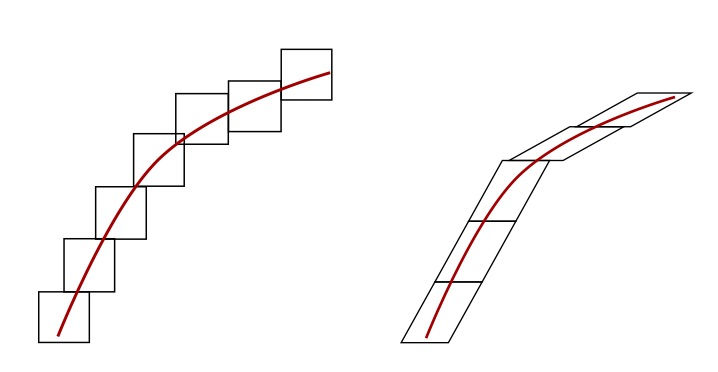
\includegraphics[width = 0.7\textwidth]{./Diagrams/anisotropic_isotropic.jpg}
\caption{Optimal covering of anisotropic scaled and sheared atoms}
\label{edges-images}
\end{figure}

\begin{figure}[!tbp]
  \centering
  \begin{minipage}[b]{0.45\textwidth}
    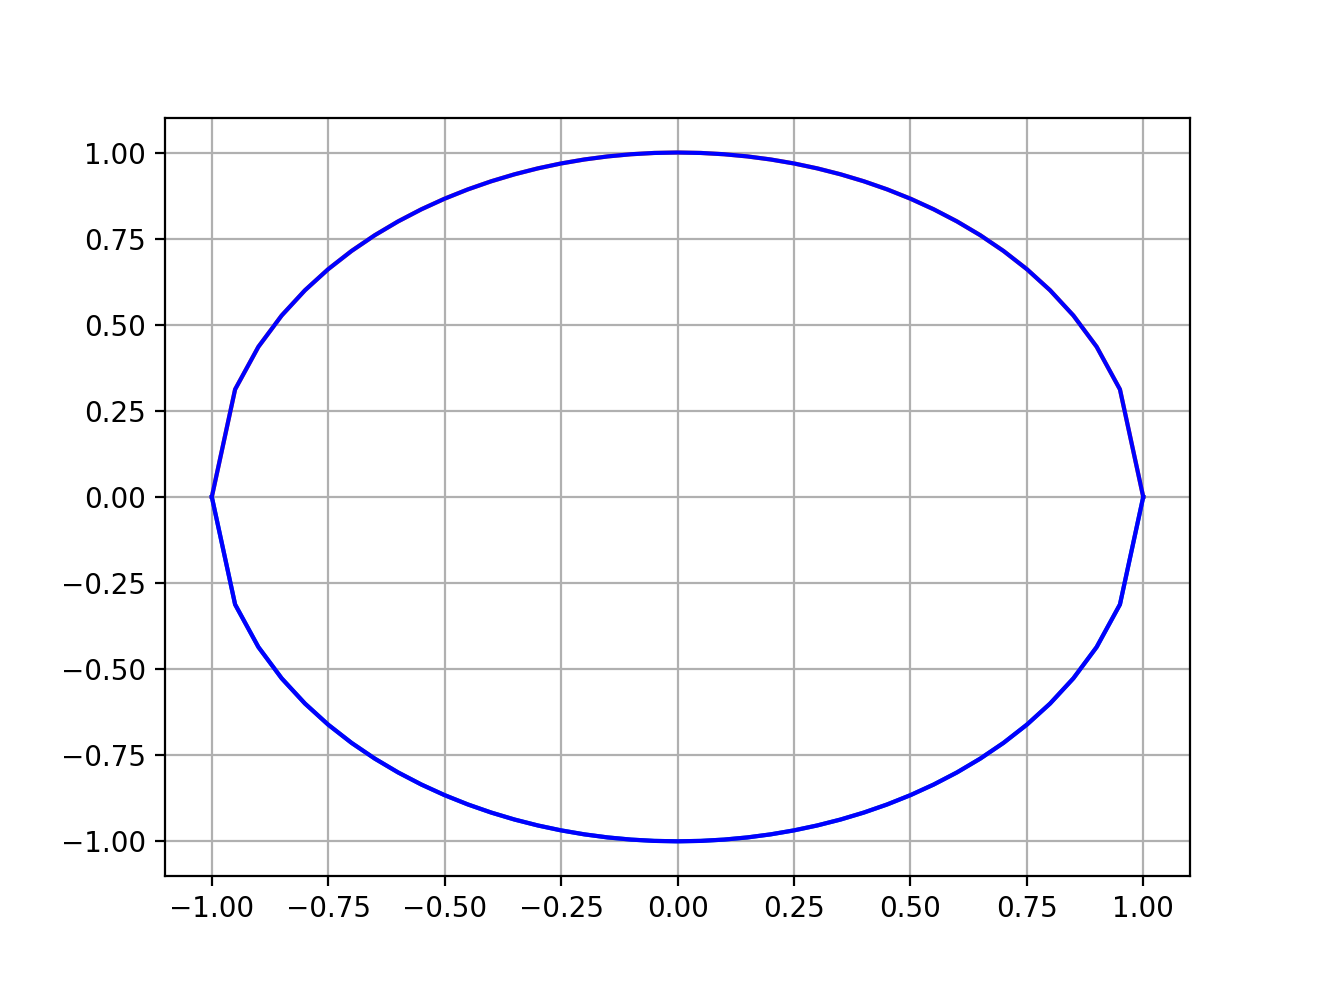
\includegraphics[width=\textwidth]{./Diagrams/circle.png}
    \caption{Circle before parabolic scaling}
  \end{minipage}
  \hfill
  \begin{minipage}[b]{0.45\textwidth}
    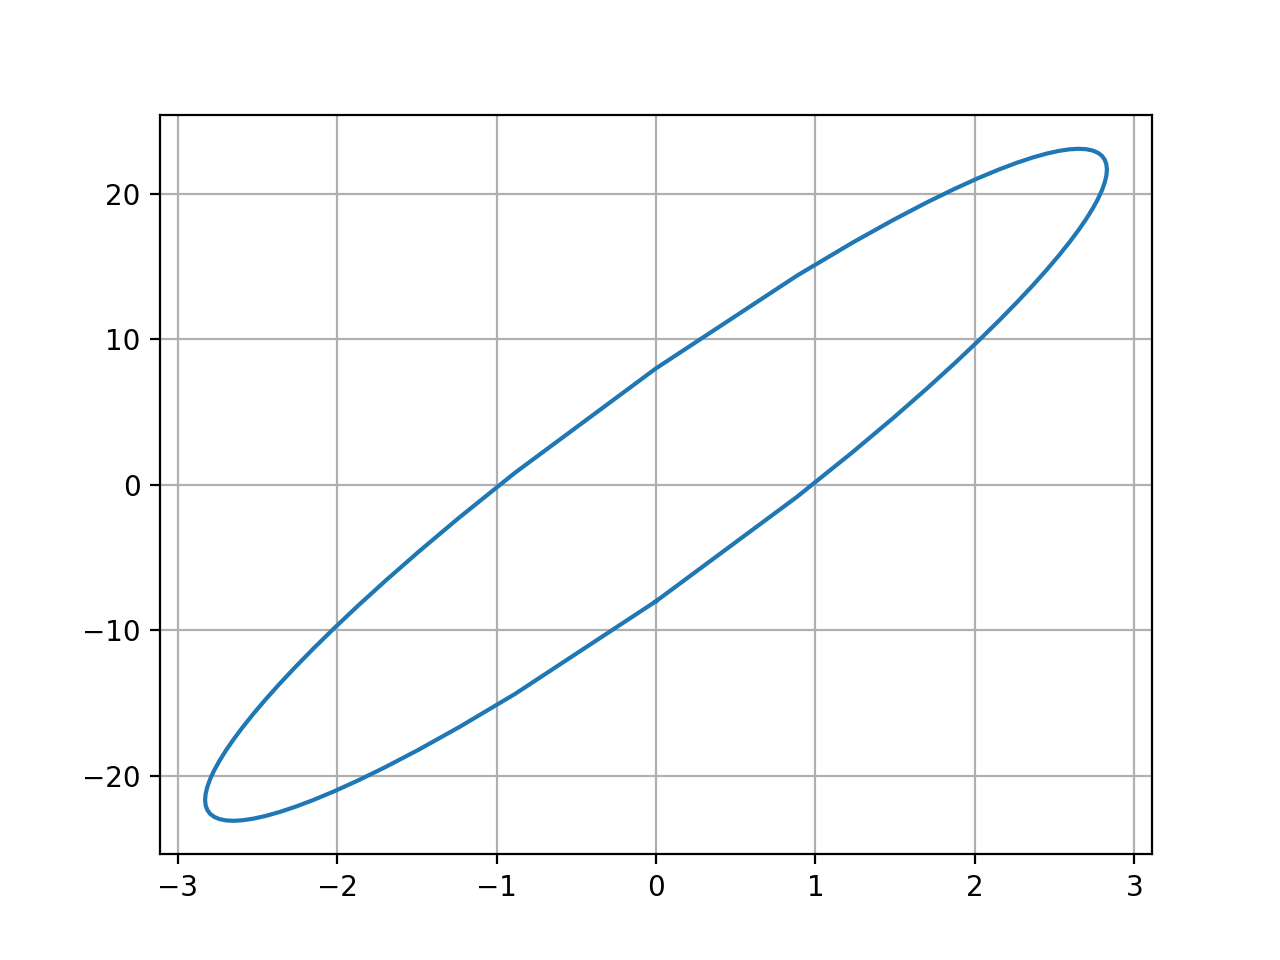
\includegraphics[width=\textwidth]{./Diagrams/circle_scaled.png}
    \caption{Circle after parabolic scaling $a=4$}
  \end{minipage}
\end{figure}


\begin{figure}[!tbp]
  \centering
  \begin{minipage}[b]{0.45\textwidth}
    
\includegraphics[width=\textwidth]{./Diagrams/square.png}
    \caption{Square before shearing}
  \end{minipage}
  \hfill
  \begin{minipage}[b]{0.45\textwidth}
    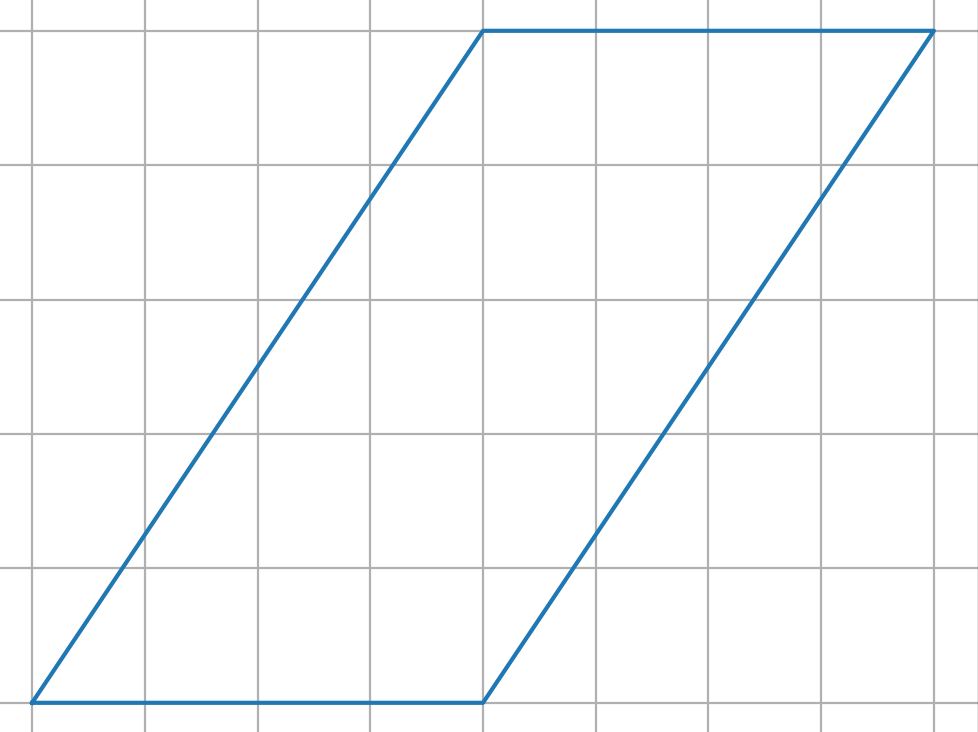
\includegraphics[width=\textwidth]{./Diagrams/square_sheared.png}
    \caption{Sheared square by a factor of $k=1$}
  \end{minipage}
\end{figure}


\begin{defn}[Continuous Shearlet Transform]
Let $\psi\in L^2(\mathbb{R}^2)$, $A_a$ and $S_s$ the parabolic scaling matrix and shearing matrix defined in~\ref{eq:scaling} and~\ref{eq:shearing} respectively, then the continuous shearlet system $SH(\psi)$ associated with $\psi$ is defined by
\begin{equation}
\label{eq:contshearletsys}
\mathcal{SH}(\psi):=\{\psi_{a,s,t}=a^{1/2}\psi (S_sA_ax-t):a\in\mathbb{R}^+,s\in\mathbb{R},t\in\mathbb{R}^2\}
\end{equation}
\end{defn}

In analogy with the discretization of wavelets, one can discretize faithfully the shearlet system which permits a straight forward implementation. We will use $a=2$ for scaling parameter since it was proven to be the best choice.

\begin{defn}[Discrete Shearlet Transform]
Let $\psi\in L^2(\mathbb{R}^2)$, $j\in\mathbb{Z}$, lets define the \textit{discrete parabolic scaling matrix} as follows

\begin{equation}
\label{eq:discscaling}
A_j:= A_2^j =
\left(\begin{matrix}
2^j & 0 \\
0 & 2^{j/2}
\end{matrix}\right)
\end{equation}

and the \textit{discrete shearing matrix} for $k\in\mathbb{Z}$

\begin{equation}
\label{eq:discshearing}
S_k:= 
\left(\begin{matrix}
1 & k \\
0 & 1
\end{matrix}\right) 
\end{equation}

Given $\psi\in L^2(\mathbb{R}^2)$, the discrete shearlet system associated with $\psi$ is defined as

\begin{equation}
\label{eq:discshearletsys}
\mathcal{DSH}(\psi):=\{\psi_{j,k,m}(x)=2^{3j/4}\psi (S_kA_jx-m):j\in\mathbb{Z},k\in\mathbb{Z},m\in\mathbb{Z}^2\}
\end{equation}
\end{defn}

It has been proven that Shearlets present a lot of features and breakthrough results; for instance they can perform common tasks of signal processing as inpainting or denoising with great results in comparison with other methods (e.g.\ wavelets); but we defined the Shearlet System with motivation on the optimal best $N$-term approximation error found by Donoho (see Theorem~\ref{C3S2T1}), and prove that this bound is reached one first need to give some definitons.

\begin{defn}[Classical shearlets]
\label{def:classical_shearlets}
Let $\psi\in L^2(\mathbb{R}^2)$ be defined by
$$
\hat{\psi}(\xi_1,\xi_2)=\hat{\psi}_1(\xi_1)\hat{\psi}_2\left(\frac{\xi_2}{\xi_1}\right)
$$
where $\psi_1,\psi_2\in L^2(\mathbb{R})$ satisfy the following properties:
\begin{itemize}
\item $\sum_{j\in\mathbb{Z}} |\hat{\psi}_1(2^{-j}\xi)|^2=1$ for a.e. $\xi\in\mathbb{R}$ (\textit{wavelet like}).
\item $\text{supp}(\hat{\psi}_1)\subseteq \left[ \frac{1}{2},-\frac{1}{16}\right]\cup\left[\frac{1}{16},\frac{1}{2}\right]$
\item $\hat{\psi}_1\in C^{\infty}(\mathbb{R})$.
\item $\sum_{k=-1,0,1}|\hat{\psi}_2(\xi+k)|^2=1$ for a.e. $\xi\in [-1,1]$ ("bump-like").
\item $\text{supp}(\hat{\psi}_2)\subseteq [-1,1]$.
\item $\hat{\psi}_2\in C^{\infty}(\mathbb{R})$.
\end{itemize}
Then, we call $\psi$ a \textit{classical shearlet}.
\end{defn}

\begin{figure}[!tbp]
  \centering
   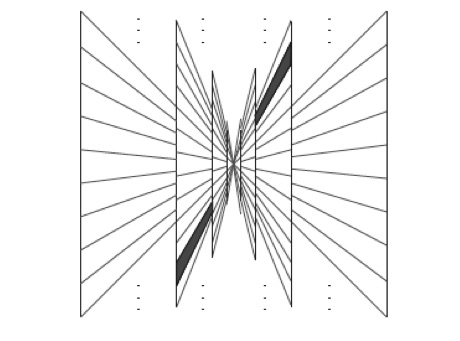
\includegraphics[width=0.7\textwidth]{./Diagrams/tiling_nocone.jpg}
    \caption{Tiling of the Fourier domain for the classical shearlets. Figure taken from \cite{Gitta-notes}, pp. 82}
  \label{fig:tiling_nocone}

\end{figure}

One can observe in Figure~\ref{fig:tiling_nocone} that the tiling of the Fourier domain of the classical shearlets is not uniform at all, it is very biased towards the $\xi_2$-axis, that will lead to some issues if one wants to analyze singularities aligned with the $x_1$-axis. For directional systems as the shearlet system one would like to have a uniform tiling of the Fourier space; to achieve this one can split the space in "cones" and associate different shearlet system for each cone. 

\bigskip

\begin{defn}[Cone-adapted shearlet system]
\label{def:cone_shearlets}
Let $\phi,\psi,\tilde{\psi}\in L^2(\mathbb{R}^2)$ and $c=(c_1,c_2)\in (\mathbb{R}^+)^2$. Lets split the Fourier space in cones $\mathcal{C}_1, \mathcal{C}_2, \mathcal{C}_3,\mathcal{C}_4$ and a central low-frequency square $\mathcal{R}$, see Figure~\ref{fig:tiling_cone}, where 
$$
\begin{aligned}
\mathcal{C}_1\cup \mathcal{C}_3 &:=\mathcal{C}_h =\{ (\xi_2,\xi_1)\in\mathbb{R}^2| |\xi_2/\xi_1|\leq 1,|\xi_1|>1\}\\
\mathcal{C}_2\cup \mathcal{C}_4 &:= \mathcal{C}_v =\{ (\xi_1,\xi_2)\in\mathbb{R}^2||\xi_2/\xi_1|> 1, |\xi_2|>1\},\\
\mathcal{R}&:=\{ (\xi_1,\xi_2)\in\mathbb{R}^2||\xi_1|,|\xi_2|\leq 1\}
\end{aligned}
$$
 

Then the \textit{cone-adapted shearlet system} associated with $\phi,\psi,\tilde{\psi}$ and $c$ is defined by 
$$
\mathcal{SH}(\phi,\psi,\tilde{\psi},c):=\mathcal{P}_{\mathcal{R}}\Phi(\phi,c_1)\cup \mathcal{P}_{\mathcal{C}_1}\Psi(\psi,c)\cup\mathcal{P}_{\mathcal{C}_2}\tilde{\Psi}(\tilde{\psi},c)
$$

where

$$
\begin{aligned}
\Phi(\phi,c_1)&:=\{\phi(x-c_1m)\text{: }m\in\mathbb{Z}\},\\
\Psi(\psi,c)&:=\{2^{3j/4}\psi(S_kA_jx-M_cm)\text{: } j\geq 0,|k|\leq\lceil 2^{j/2}\rceil,m\in\mathbb{Z}^2\},\\
\tilde{\Psi}(\tilde{\psi},c)&:=\{2^{3j/4}\tilde{\psi}(\tilde{S}_k\tilde{A}_jx-\tilde{M}_cm)\text{: } j \geq 0,|k|\leq\lceil 2^{j/2}\rceil,m\in\mathbb{Z}^2\},
\end{aligned}
$$

with 

$$
M_c=\left(\begin{matrix} c_1 & 0 \\ 0 & c_2\end{matrix}\right)\text{,  }
\tilde{M}_c=\left(\begin{matrix} c_2 & 0 \\ 0 & c_1\end{matrix}\right) \text{,  }
\tilde{S}_k=\left(\begin{matrix} 1 & 0 \\ k & 1 \end{matrix}\right)\text{,  }
\tilde{A}_j=\left(\begin{matrix} 2^{j/2} & 0 \\ 0 & 2^j\end{matrix}\right)
$$

and $P_{\mathcal{R}}$, $\mathcal{P}_{\mathcal{C}_1}$ and $\mathcal{P}_{\mathcal{C}_2}$ are the projections in the Fourier domain.
\end{defn}

\begin{figure}[!tbp]
  \centering
   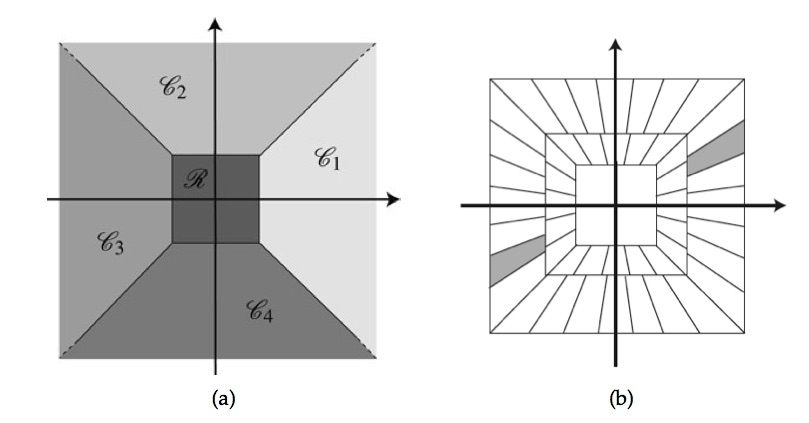
\includegraphics[width=0.9\textwidth]{./Diagrams/tiling_cone.jpg}
    \caption{(a) Tiling of the Fourier domain into cones. (b) Frequency tiling generated by cone-adapted shearlets. Figure taken from \cite{Gitta-notes} pp. 83 }
  \label{fig:tiling_cone}
\end{figure}

\bigskip

In the case of the wavelet transform the discretization and implementation of the algorithm that performs it is straight-forward since dilation can be performed by subsampling and one can use fourier transform properties to translate convolution into multiplication and that can be implemented optimally with the fft-algorithm. One can also take in account that the convolution operation with a function of compact support can be thought as a filtering operation in signal processing, so a wavelet system and a multeresolution analysis  is interpreted in the typical implemenation as a filter bank, the last using a high pass and a low pass filter that characterize the interaction of the wavelet and scaling function, the former obeying the admissibility condition. 

\bigskip

For the same reasons the Shearlet Transform of a function $f\in L^2(\mathbb{R}^2)$, defined by its coefficients $\langle f,\psi_{j,k,m}\rangle$ has a faithfull implementation using filtering and subsampling operations just taking care of the invariance of the $\mathbb{Z}^2$ grid under the discretization of the shearing operator (Wang-Q. Lim proposed a solution for this on \cite{Nonseparableshear}); the filters need to characterize the functions $\phi$ and $\psi$ on the cone-adapated shearlet system (Definition~\ref{def:cone_shearlets}). The simplest choice is to take $\psi$ to be the tensor product of a wavelet function $\psi_1$ and a scaling function $\phi_1$ related to a multiresolution analysis, this approach is known as the separable shearlet transforms with generating functions:

$$
\begin{aligned}
\phi(x_1,x_2)&=\phi_1(x_1)\phi_1(x_2)\\
\psi(x_1,x_2)&=\psi_1(x_1)\phi_1(x_2)
\end{aligned}
$$

Even this separable approach forms a frame a frame for $L^2(\mathbb{R}^2)$ (check Section~\ref{sec:ShearletsFrames} for a detail explanation) and simplifies the implementation, it is not a good choice for directional representations; the separability causes a significant overlap between $\text{supp}(\hat{\psi}_{j,k,m})$ and $\text{supp}(\hat{\psi}_{j,k+1,m})$, see Figure~\ref{fig:separable_nonseparable}. Also in Figure~\ref{fig:separable_nonseparable} one can see that wedge shaped support is well adapted for covering the frequency domain by the application of the shear and scale operator while improving directional selectivity to achieve this Wang-Q. Lim proposed in 2013 a non-separable shearlet generator $\psi^{\text{non}}$ given by the relation

$$
\hat{\psi}^{\text{non}}(\xi)=P\left(\frac{\xi_1}{2},\xi_2\right)\hat{\psi}(\xi),
$$

where $\psi$ is the already mentioned separable shearlet generator and $P$ is a 2D directional fan filter (see \cite{Nonseparableshear} for a more detailed explanation of this filter). The wedge form that non-separable shearlet generators give to the shearlet system the ability to cover the Fourier domain optimally. We will use this approach in this thesis; the implementation of the non-separable shearlet transform is widely explained in \cite{Shearlab} where the most known implemenation is based on, Shearlab3D in matlab (one can download it in \url{https://shearlab.org}); by the improvement of performance we will use the Julia Programming Language (\url{https://julialang.org/}) implementation of this library that can be downloaded in \url{https://github.com/arsenal9971/Shearlab.jl} or installed from the Julia REPL using \lstinline[language=julia]{Pkg.add("Shearlab")}.

\begin{figure}[h!]
\centering
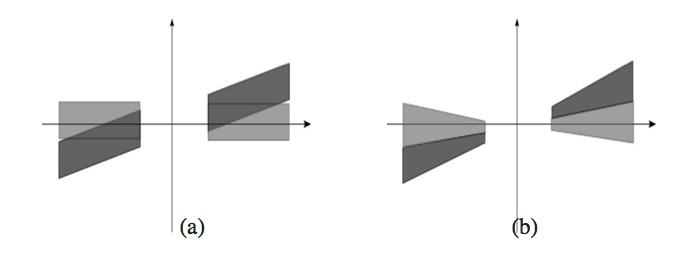
\includegraphics[width=0.8\textwidth]{./Diagrams/separable_nonseparable.jpg}
\caption{Frequency covering by shearlets $\psi_{j,0,m}$ and $\psi_{j,1,m}$ (a) with separable generator (b) with non-separable generator. Figure taken from \cite{Nonseparableshear} pp. 12}
\label{fig:separable_nonseparable}
\end{figure}

We finally can give in this section the result that we were looking for to justify formally the superiority of the Shearlet System over the Wavelet System on representating optimally the \textit{cartoon-like functions}, we will again make use of the term frame, despite it has not been introduced yet, but until the next section.

\begin{thm}
\label{thm:optimal_shearlets}
Let $\psi\in L^2(\mathbb{R}^2)$ be compactly supported.

Assume that  for $\alpha>5$, $\gamma\geq 4$, $q>q'>0$ and $q>r>0$, it holds that
\begin{equation}
\label{eq:boundframe}
|\hat{\psi}(\xi_1,\xi_2)|\leq C \min\{1,|q\xi_1|^{\alpha}\}\min\{1,|q'\xi_1|^{-\gamma}\}\min\{1,|r\xi_2|^{-\gamma}\}
\end{equation}
for some constant $C>0$ and that for $h\in L^1(\mathbb{R}^1)$ 
$$
|\frac{\partial}{\partial\xi_2}\hat{\psi}(\xi)|\leq |h(\xi_1)|\left(1+\big| \frac{\xi_2}{\xi_1}\big|\right)^{-\gamma}
$$
is satisfied. Assume that the same conditions are satisfied for $\tilde{\psi}$. Then, if the \textit{cone-adapated shearlet system} on definition~\ref{def:cone_shearlets} $\mathcal{SH}(\phi,\psi,\tilde{\psi},(1,1))$ forms a frame for $L^2(\mathbb{R}^2)$, then there exists a constant $C'>0$ such that for all $f\in\mathcal{E}^2(\mathbb{R}^2)$, we have 

\begin{equation}
\label{eq:optimalshearlets}
\sigma_N(f,\mathcal{SH}(\phi,\psi,\tilde{\psi},(1,1))\leq C'N^{-1}(\log N)^{3/2} \text{as  } N\longrightarrow\infty
\end{equation}
\end{thm}
\begin{proof}
The proof of this theorem is quite technical and it has not a great impact on the results of our thesis, so one will let the reader to consult \cite{FirstShearlets} for a detailed proof. 
\end{proof}

As $N$ goes bigger the logarithm in the estimate~\ref{eq:optimalshearlets} can be taken as a constant, so Theorem~\ref{thm:optimal_shearlets} shows that the Cone-Adapted Shearlet System atains the theoretical optimal best $N$-term approximation error for the cartoon like functions given in Theorem~\ref{C3S2T1}. Cartoon-like functions represent accurately natural images, so this system is proven to be a great option to inpaint EPIs in this thesis. In the next sections we will show other features of the Shearlets as its character of frames for $L^2(\mathbb{R}^2)$ as well as other forms of them using general scaling matrix, called alpha shearlets and we will show why a particular case of alpha shearlets is the best to inpaint sparse-sampled EPIs.

\section{Shearlets as Frames}
\label{sec:ShearletsFrames}

Lets now take a bigger picture on representation systems. An orthonormal basis for Hilbert space $\mathcal{H}$ is a sequence $(\phi_i)_{i\in I}\subset\mathcal{H}$ such that for each vector $x\in\mathcal{H}$
\begin{equation}
\label{eq:parseval}
x=\sum_{i\in I}\langle x,\phi_i\rangle \phi_i
\end{equation}

so one can represent each vector in terms of the collection and one can decompose each element $x\in\mathcal{H}$ as
$$
x\mapsto (\langle x,\phi_i\rangle)_{i\in I}\text{,  }\mathcal{H}\longrightarrow \ell_2(I)
$$

even this two features (decomposition and recovery) are very simply expressed for orthonormal bases, one woul like to extend the theory for different reasons. For example, it is not possible to recover $x$ if one loses some of the coefficients $\langle x, \phi_i\rangle$, so the induced decomposition is not robust. In the last section we mentioned the imporance of sparse representation of signals in different applications, but an orthonormal basis forces the representation coefficients to be $\langle x,\phi_i\rangle$, the sequence of coefficients will not have a rapid decay. One will call this two mentioned characteristics as \textit{Robust Decomposition}, and \textit{Sparse representation}. 

\bigskip

A natural generalization of the concept of orthonormal bases is the concept of frames, to define them one weakens the Parseval equation~\ref{eq:parseval}.

\bigskip

\begin{defn}[Frames]
\label{def:frames}
\begin{enumerate}
\item[(1)] A sequence $(\phi_i)_{i\in I}$ in a Hilbert space $\mathcal{H}$ is called a \textbf{frame} for $\mathcal{H}$, if there exist constans $0<A\leq B<\infty$ such that
\begin{equation}
\label{eq:frames}
A||x||^2\leq \sum_{i\in I}|\langle x,\phi_i\rangle|^2\leq B||x||^2 \text{,  }\forall x\in \mathcal{H}
\end{equation}
$A$ and $B$ are called lower and upper frame bound.
\item[(2)] If $A$ and $B$ can be chosen to be equal, we call it ($A$-) tight frame. If $A=B=1$ is possible, $(\phi_i)_{i\in I}$ forms a Parseval frame.
\item[(3)] If only the upper bound in~\ref{eq:frames} holds, we call $(\phi_i)_{i\in I}$ a Bessel sequence.
\end{enumerate}
\end{defn}

\bigskip

With this definition an orthonormal basis will be a Parseval frame. Since $A>0$ frames also span the whole space $\mathcal{H}$, frames allows one to obtain both characteristics \textit{robust decomposition} and \textit{sparse representation}; for a detailed explanation of this we highly recommend the Chapter 5 of \cite{Mallat}.

\bigskip

In the last section we introduced different representation systems for signals in $L^2(\mathbb{R}^2)$, as Gabor systems that emerge motivated by the short time fourier transform, wavelet and shearlet systems. This systems will form a frame under certain conditions on the generating functions and parameters. For example in the case of wavelet systems we have the next theorem that gives a necessary condition to form frames.

\bigskip

\begin{thm}[Necessary condition for wavelet frames]
Let $a>1$, $b>0$ and $\psi\in L^2(\mathbb{R})$ a wavelet function such that the related system $W(\psi,a,b)$ forms a frame for $L^2(\mathbb{R})$ with frame bounds $A$ and $B$. Then, we have
$$
A\leq \frac{1}{b}\sum_{j\in\mathbb{Z}}|\hat{\psi}(a^j\xi)|^2\leq B \text{,   }\forall\xi\in\mathbb{R}
$$
\end{thm}
\begin{proof}
One can find the proof in Theorem 3.3 of \cite{daubechies}
\end{proof}

\bigskip

Sufficient conditions of wavelet frames are more technical and one can find them in Theorem 3.15 of \cite{Gitta-notes}. In our case we would like to know under what conditions \textit{Classical Shearlets} and \textit{Cone-adapted shearlets} separable and nonseparable form frames, and for that we have the next results.

\begin{thm}
Let $\psi$ be a classical shearlet, i.e.\ obeys the conditions~\ref{def:classical_shearlets}. Then the associated wavelet system $\mathcal{SH}(\psi)$ forms a Parseval frame for $L^2(\mathbb{R}^2)$.
\end{thm}
\begin{proof}
By the above properties of $\psi_1$ and $\psi_2$, we have
$$
\begin{aligned}
\sum_{j\in\mathbb{Z}}\sum_{k\in\mathbb{Z}}|\hat{\psi}(S^T_{-k}A_{-j}\xi)|^2&=\sum_{j\in\mathbb{Z}}|\hat{\psi}_1(2^{-j}\xi_1)|^2\sum_{k\in\mathbb{Z}}|\hat{\psi}_2(2^{j/2}\xi_2/\xi_1-k)|^2\\
&=\sum_{j\in\mathbb{Z}}|\hat{\psi}_1(2^{-j}\xi_1)|^2=1
\end{aligned}
$$
this holds for almost every $\xi\in\mathbb{R}^2$, using on this equation Plancherel's and Parseval's identity is enough to finish the proof.
\end{proof}

Using a similar proof of the last theorem one can prove the next theorem.

\begin{thm}
Let $\psi\in L^2(\mathbb{R}^2)$ be a classical shearlet. Then 
$$
\Psi(\psi,(1,1)):=\{2^{3j/4}\psi(S_kA_jx-m)\text{: }j\geq 0,|k|\leq\lceil 2^{j/2}\rceil,m\in\mathbb{Z}^2\}
$$
forms a Parseval frame for 
$$
\{f\in L^2(\mathbb{R})\text{:  supp}\hat{f}\subset\{\xi\in\mathbb{R}^2\text{:  }|\xi_1|\geq 1,|\xi_2/\xi_1|\leq 1\}\}
$$
\end{thm}

Finally one can state the result for the \text{cone-adapted shearlet system}.

\begin{thm}
For $\alpha >\gamma>3$, $q>q'>0$ and $q>r>0$, let 
\begin{equation}
\label{eq:coneshearframes}
|\hat{\psi}(\xi_1,\xi_2)|\leq C\min\{1,|q\xi_1|^{\alpha}\}\min\{1,|q'\xi_1|^{-\gamma}\}\min\{1,|r\xi_2|^{-\gamma}\}
\end{equation}
for some constant $C>0$, and that

$$
\sum_{j,k\in\mathbb{Z}}|\hat{\psi}(S^T_{-k}A_{-j}\xi)|^2\geq C'>0
$$

for almost every $\xi\in\mathbb{R}^2$. For $\tilde{\psi}$, we assume similar conditions. Then, there exists some $c_0$ such that $\mathcal{SH}(\phi,\psi,\tilde{\psi},c)$, with suitable $\phi$, forms a frame for $L^2(\mathbb{R}^2)$ for all $c_1,c_2<c_0$ and for the frame bounds, we have 

$$
C_1(\alpha,\gamma,q,q',r,c_1,c_2)\leq A\leq B\leq C_2(\alpha,\gamma,q,q',r,c_1,c_2)
$$

\end{thm}
\begin{proof}
We refer to \cite{FirstShearlets} for the proof of this theorem. 
\end{proof}

The choice of functions $\psi$ and $\phi$ presented in the last section in both separable and non-separable fashion obey the inequality~\ref{eq:coneshearframes} (see \cite{Nonseparableshear}); therefore the related shearlet system will form a frame. This machinery shows the strong properties of the shearlet systems being frames, presenting both sparse representation and robust decomposition and in particular shows that the shearlets will span $L^2(\mathbb{R}^2)$. In the next section we will extend the notion of scaling that is suitable for levels of anisotropy. 

\section{Universal Shearlets and $\alpha$-Shearlets}
\label{sec:AlphaShearlets}

The classical and the cone-adapted shearlets that we mentioned so far make use of a parabolic scaling matrix to perform the scaling operation, this matrix has the form 

\begin{equation}
\label{eq:parabolic_scaling}
A_j=\left(
\begin{matrix}
2^j & 0 \\
0 & 2^{j/2}
\end{matrix}
\right)
\end{equation}

the form of the matrix has been motivated by the aim to construct best approximation of functions with singularities over parabolic curves, but one would like to have more flexibility on curves that dominate the images; in the case of the Epipolar Images as one can see in Section~\ref{sec:Epi-geometry} one would like to have a system that is good to approximate straight line singularities. 

\bigskip

The natural generalization of the parabolic scaling was motivated by the inpainting problem (see \cite{Gitta-alpha}) is reached by the introduction the so called \textit{scaling sequences} $(\alpha_j)_j\subseteq (-\infty,2)$ with associated scaling matrices

\begin{equation}
\label{eq:alpha_scaling}
A_{j,\alpha_j,(h)}=\left(
\begin{matrix}
2^j & 0 \\
0 & 2^{\alpha_j j/2}
\end{matrix}
\right)
\end{equation}

which offers a lot of flexibility in scaling and let us choose the level of anisotropy for each scale $j$ independently; using definition of scaling matrix we will define the \textit{Universal Shearlet System} introduced by Gitta Kutyniok and Martin Genzel in \cite{Gitta-alpha}; it is very convinient to generalize the notion of scaling also because it permits us to have a uniform treatment of different band-limited systems like classical cone-adapted shearlets, ridgelets and band-limited wavelets. 

\bigskip

One main objective of the introduction of the \textit{Universal Shearlet System} is to construct due to its flexibility a compactly supported directional system which forms a Parseval frame and gives an optimal sparsifying approximation of cartoon-like functions. The classical shearlet theory showed that certain class of band-limited shearlets constitute a Parseval frame and provide an optimal sparse approximation (see \cite{Guo-Labate}); but, when trying to force the compact support of those even under certain conditions optimal approximation rates can be achieved, they weill not have the Parseval property. 

\bigskip 

Lets proceed with the construction of the \textit{Universal Shearlets}. First let us recall the definition of the \textit{Schwartz functions space} 

$$
\mathbb{S}(\mathbb{R}^d):=\{\phi\in C^{\infty}(\mathbb{R}^d)|\forall K,N\in\mathbb{N}_0:\sup_{x\in\mathbb{R}^d}(1+|x|^2)^{-N/2}\sum_{|\alpha|\leq K}|D^{\alpha}\phi(x)|<\infty\}
$$

we will rather use the compact notation $\langle|x|\rangle:=(1+|x|^2)^{-N/2}$, the fourier transform will be an operator of $\mathbb{S}(\mathbb{R}^d)$. 

\bigskip

Lets define a scaling function as  $\phi\in\mathbb{S}(\mathbb{R})$ satisfying $0\leq \hat{\phi}\leq 1$, $\hat{\phi}(u)=1$ for $u\in [-1/16,1/16]$, and $\text{supp}(\hat{\phi})\subset [-1/8,1/8]$. A function with these properties is usually named \textit{Meyer scaling function}. Now, lets define the \textit{corona scaling function} for $j\in\mathbb{N}_0$ by ($\xi=(\xi_1,\xi_2)\in\mathbb{R}^2$)

$$
\begin{aligned}
\hat{\Phi}(\xi)&:=\hat{\phi}(\xi_1)\hat{\phi}(\xi_2),\\
W(\xi)&:= \sqrt{\hat{\Phi}^2(2^{-2}\xi)-\hat{\Phi}^2(\xi)},\\
W_j(\xi)&:=W(2^{-2j}\xi).
\end{aligned}
$$

The functions $W_j$ are compactly supported in corona-shaped scaling levels, i.e.\,
\begin{equation}
\label{eq:alpha31}
\text{supp}W_j\subset \mathcal{K}_j:=[-2^{2j-1},2^{2j-1}]^2\setminus (-2^{2j-4},2^{2j-4})^2
\end{equation}

and as in the case of classical cone-adapted shearlets one can decompose the Fourier domain by the sequence of scaling functions:

$$
\hat{\Phi}^2(\xi)+\sum_{j\geq 0} W^2_j(\xi)=1\text{,   }\xi\in\mathbb{R}^2
$$ 

as in the definiton of the classical shearlets the function $W$ can be viewed as a wavelet, in the same manner one considers a \textit{bump-like} function $v\in C^{\infty}(\mathbb{R})$ which satisfies $\text{supp}v\subset [-1,1]$ and 

\begin{align}
& |v(u-1)|^2+|v(u)|^2+|v(u+1)|^2 = 1 \quad \textrm{for} \quad u\in[-1,1] \quad \textrm{,and}\label{eq:alpha33}\\
& v(0)=1 \quad \textrm{and} \quad v^{(n)}(0)=0\quad\textrm{for}\quad n\geq 1\label{eq:alpha34}
\end{align}

For an explicit construction of $v$ we refer to \cite{Guo-Labate}, again to avoid directional bias along $\xi_2$-axis at the Fourier space we will use the cone-adapted approach (see definition~\ref{def:cone_shearlets}), with 

$$
\begin{aligned}
\mathcal{C}_{(h)} &:=\{ (\xi_1,\xi_2)\in\mathbb{R}^2||\xi_2/\xi_1|\leq 1\}\\
\mathcal{C}_{(v)} &:=\{ (\xi_1,\xi_2)\in\mathbb{R}^2||\xi_2/\xi_1|>1\}
\end{aligned}
$$

\begin{figure}[h!]
\centering
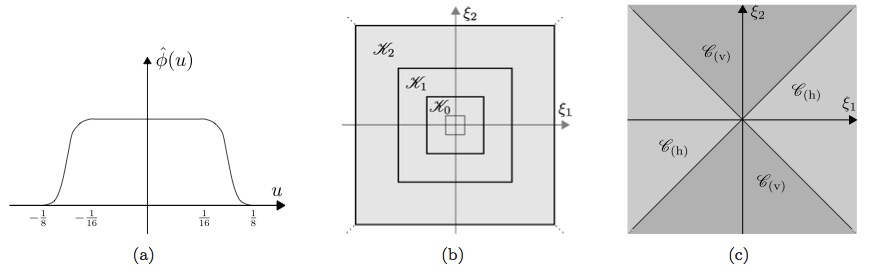
\includegraphics[width=0.9\textwidth]{./Diagrams/alphapartcones.jpg}
\caption{(a) Fourier transform of a Meyer scaling function. (b) Decomposition of the frequency plane by corona functions $W_j$ and $\Phi$. (c) Symmetric frequency decompositionby cones. Figure taken from \cite{Gitta-alpha} pp. 11}
\label{fig:separable_nonseparable1}
\end{figure}

Lets introduce adapted versions of the usual shearing and scaling matrices,
$$
A_{\alpha,(h)}:=\left(\begin{matrix} 2 & 0 \\ 0 & 2^{\alpha/2}\end{matrix}\right) \quad \textrm{,}\quad S_{(h)}:=\left(\begin{matrix} 1 & 1\\ 0 & 1\end{matrix}\right)
$$
$$
A_{\alpha,(v)}:=\left(\begin{matrix}2^{\alpha/2} & 0 \\ 0 & 2 \end{matrix}\right)\quad \textrm{,}\quad S_{(v)}:=\left(\begin{matrix} 1 & 0 \\ 1 & 1\end{matrix}\right)
$$

where $\alpha\in (-\infty,2)$ is the \textit{scaling parameter}, $A_{j,\alpha,(\iota)}:=A^j_{\alpha,(\iota)}$ and $S_{k,(\iota)}:=S^k_{(\iota)}$ for $\iota\in\{h,v\}$. The adapted \textit{cone functions} are given by
$$
V_{(h)}(\xi):=v(\xi_2/\xi_1)\textrm{,}\quad V_{(v)}(\xi):=v(\xi_1/\xi_2)\textrm{,}\quad \xi\in\mathbb{R}^2.
$$
Lets define now the ingredients of a universal shearlet system.

\bigskip

\begin{defn}
\label{def:alpha31}
Let $\Phi$, $W$, $V_{(h)}$, $V_{(v)}\in L^2(\mathbb{R}^2)$ be defined as before.
\begin{enumerate}
\item[1.] \textbf{Coarse scaling functions}: For $k\in\mathbb{Z}^2$, we set 
$$
\psi_{-1,k}:=\Phi(x-k)\textrm{,}\quad x\in\mathbb{R}^2.
$$
\item[2.] \textbf{Interior shearlets}: Let $\alpha\in (-\infty,2)$, $j\in\mathbb{N}_0$, $k\in\mathbb{Z}$ with $|k|< 2^{(2-\alpha)j/2}$, $m\in\mathbb{Z}^2$ and $\iota\in\{h,v\}$. The shearlets will be given by 

\begin{equation}
\label{eq:alpha35}
\hat{\psi}^{\alpha,(\iota)}_{j,k,m}(\xi):=2^{-(\alpha+2)j/4}W(2^{-j}\xi)V_{(\iota)}(\xi^{\top} A_{-j,\alpha,(\iota)}S_{-k,(\iota)})e^{-2\pi i\xi^{\top}A_{-j,(\iota)}S_{-k,(\iota)}}\textrm{,}\quad \xi\in\mathbb{R}^2
\end{equation}

\item[3.] \textbf{Boundary shearlets}: For $\alpha\in(-\infty,2)$, $j\geq 1$, $k=\pm\lceil 2^{(2-\alpha)j/2}\rceil$ and $k\in\mathbb{Z}^2$, we define
\begin{equation}
\label{eq:alpha36}
\hat{\psi}_{j,k,m}^{\alpha}:=
\begin{cases}
2^{-(\alpha+2)j/4-1/4}W(2^{-j}\xi)V_{(h)}(\xi^{\top} A_{-j,\alpha,(h)}S_{-k,(\iota)})e^{-\pi i\xi^{\top}A_{-j,\alpha,(h)}S_{-k,(h)}m}\textrm{,}\quad \xi\in\mathcal{C}_{(h)},\\
2^{-(\alpha+2)j/4-1/4}W(2^{j}\xi)V_{(v)}(\xi^{\top}A_{-j,\alpha,(v)}S_{-k,(v)})e^{-\pi i\xi^{\top}A_{-j,\alpha,(v)}S_{-k,(h)}m}\textrm{,}\quad \xi\in\mathcal{C}_{(v)}
\end{cases}
\end{equation}
and in the case $j=0$, $k=\pm 1$, we define
$$
\hat{\psi}^{\alpha}_{0,k,m}:=
\begin{cases}
W(\xi) V_{(h)}(\xi^{\top}S_{-k,(h)})e^{-2\pi i\xi^{\top}m}\textrm{,}\quad \xi\in\mathcal{C}_{(h)}\textrm{,}\\
W(\xi)V_{(v)}(\xi^{\top}S_{-k,(v)})e^{-2\pi i\xi^{\top}m}\textrm{,}\quad \xi\in\mathcal{C}_{(v)}.
\end{cases}
$$
One can compare this definition of shearlet system with the Definition~\ref{def:cone_shearlets} of classical cone-adapted shearlet system and see that in the case of $\alpha = 1$ both are the same. The Fourier transform $\hat{\psi}_{j,k,m}^{\alpha,(h)}$ has compact support in the trapezoidal region

\begin{equation}
\label{eq:alpha37}
\{\xi\in\mathbb{R}^2|\xi_1\in[-2^{j-1},2^{j-1}]\setminus (-2^{j-2},2^{j-2}),||\xi_2/\xi_1-k2^{-(2-\alpha)j/2}|\leq 2^{-(2-\alpha)j/2}\}.
\end{equation}
\end{enumerate}
\end{defn}

\bigskip

Since the boundary shearlets were defined piecewise, smoothness (of the Fourier transforms) is not guaranteed for all $\alpha\in (-\infty,2)$. The exponent $2^{(2-\alpha)j/2}$ needs to be necessarily integer-valued when analyzing the first partial derivatives of eq.~\ref{eq:alpha36}. To satisfy this for every $j\in\mathbb{Z}$, we would have to restrict the set of admissible $\alpha$ to the set of integers; but this would not give us the arbitrary scaling behavior that we are looking for. To overcome this issue one can relax the condition of a globally fixed $\alpha$ and, introduce a \textit{separate} scaling parameter $\alpha_j$ on each scale. The universal shearlet system will be associated with a whole sequence $(\alpha_j)_{j\in\mathbb{N}_0}\subset\mathbb{R}$. In this setting the set of admissible scaling parameters can be substantially enlarged since we have $(2-\alpha_j)j/2\in\mathbb{Z}$ whenever $\alpha_j$ is multiple of $2/j$. 

\bigskip

\begin{defn}
\label{def:alpha32}
A sequence $(\alpha_j)_{j\in\mathbb{N}_0}\subset\mathbb{R}$ is called a scaling sequence if 
$$
\alpha_j\in A_j:=\left \{\frac{2n}{j}\big| n\in\mathbb{Z},n\leq j-1\right \}=\left \{\ldots,-\frac{4}{j},-\frac{2}{j},0,\frac{2}{j},\ldots,1-\frac{2}{j}\right \}
$$
\end{defn}

\bigskip

\begin{defn}
\label{def:alpha33}
Let $(\alpha_j)_{j\in\mathbb{N}_0}$ be a \textit{scaling sequence}. Then we define the associated universal-scaling shearlet system, or shorter, universal shearlet system, by
$$
\mathcal{SH}(\phi,v,(\alpha_j)_j):=\mathcal{SH}_{\text{Low}}(\phi)\cup\mathcal{SH}_{\text{Int}}(\phi,v,(\alpha_j)_j)\cup\mathcal{SH}_{\text{Bound}}(\phi,v,(\alpha_j)_j),
$$
where
$$
\begin{aligned}
\mathcal{SH}_{\text{Low}}(\phi)&:=\{\psi_{-1,m}|m\in\mathbb{Z}^2\}\\
\mathcal{SH}_{\text{Int}}(\phi,v,(\alpha_j)_j)&:=\{\psi_{j,k,m}^{\alpha_j,(\iota)}|j\geq 0,|m|< 2^{(2-\alpha_j)j/2},m\in\mathbb{Z}^2,\iota\in\{h,v\}\},\\
\mathcal{SH}_{\text{Bound}}(\phi,v,(\alpha_j)_j)&:=\{\psi_{j,k,m}^{\alpha_j}|j\geq 0,|k|=\pm 2^{(2-\alpha_j)j/2},m\in\mathbb{Z}^2\}.
\end{aligned}
$$

\end{defn}

\bigskip

Since the elements of a scaling sequence $\alpha_j$ can be chosen independently for each scaling level and, in particular, the sequence $(\alpha_j)_j$ does not need to converge; this permits a faithful implementation of the universal shearlet transform; this is already implemented in the toolbox used in this thesis (Shearlab.jl) one determines the total number of shearings (on each scale) first given by $|k|\leq \lceil 2^{(2-\alpha_j)j/2}\rceil$, rather that selecting a fixed $\alpha_j$. We are ready to prove the main property of the universal shearlet system, i.e.\ its character of frame.

\begin{thm}[Universal shearlet frames]
\label{thm:alpha34}
Let $(\alpha_j)_{j}$ be a scaling sequence and $\mathcal{SH}(\phi,v,(\alpha_j)_j)$ be an associated universal shearlet system. Then $\mathcal{SH}(\phi,v,(\alpha_j)_j)$ constitutes a Parseval frame for $L^2(\mathbb{R}^2)$ consisting of band-limited Schwartz functions. Moreover, the interior and boundary shearlets have infinitely  many vanishing moments. 
\end{thm}
\begin{proof}
Lets proceed with the proof of the different properties required.
\begin{itemize}
\item\textit{Band-limiting and vanishing moment property:} Observing that $(0,0)\notin \text{supp}W_k\subset \mathcal{K}_j$ which immediately follows from Definition~\ref{def:alpha31}.
\item\textit{Smoothness:} Due to the band-limiting of $\mathcal{SH}(\phi,v,(\alpha_j)_j)$, it is sufficient to show that the Fourier transforms of the elements are smooth. This will imply that $\mathcal{SH}(\phi,v,(\alpha_j)_j)\subset \mathbb{S}(\mathbb{R}^2)$. 

\bigskip

The smoothness of $\mathcal{SH}_{\text{Low}}(\phi,v,(\alpha_j)_j)$ and $\mathcal{SH}_{\text{Int}}(\phi,v,(\alpha_j)_j)$ are induced by their smooth defining functions $\phi$ and $v$. We still need to consider elements $\psi^{\alpha_j}_{j,k,m}\in\mathcal{SH}_{\text{Bound}}(\phi,v,(\alpha_j)_j)$. In the interior of $\mathcal{C}_{(h)}$ and $\mathcal{C}_{(v)}$, the smoothness is again obvious. Thus, we only need to analyze the boundary lines of the cones which are given by $\{|\xi_1|=|\xi_2|\}$.

\bigskip

Lets use the shortcut $k_j:=2^{(2-\alpha_j)j/2}$ for the maximal shearing number (on scale $j$) and simplify the definition of $\hat{\psi}_{j,k,m}^{\alpha_j}$ (for $j\geq 1$):

\begin{equation}
\label{eq:alpha71}
\hat{\psi}^{\alpha_j}_{j,k,m}(\xi)=2^{-\frac{(2+\alpha_j)j}{4}-\frac{1}{4}}\cdot
\begin{cases}
W(2^{-j}\xi)v(k_j(\xi_2/\xi_1-1))&e^{-\pi i[2^{-j}\xi_1 m_1+2^{-\alpha_j j/2}(\xi_2-\xi_1)m_2]}\\
& \textrm{,}\quad \xi\in\mathcal{C}_{(h)},\\
W(2^{-j}\xi)v(k_j(\xi_1/\xi_2-1))&e^{-\pi i[2^{-j}\xi_1 m_1+2^{-\alpha_j j/2}(\xi_1-\xi_1)m_2]}\\
&\textrm{,}\quad \xi\in\mathcal{C}_{(v)},
\end{cases}
\end{equation}

In the case of $\xi_1=\pm \xi_2$, both terms coincide implying the continuity of $\hat{\psi}_{j,k,m}^{\alpha_j}$. By the same argument, the continuity of $\hat{\psi}_{j,-k_j,m}^{\alpha_j}$ is verified. Next we compute the partial derivatives of both terms in eq.~\ref{eq:alpha71} which are given by

\begin{equation}
\label{eq:alpha72}
\begin{aligned}
\frac{\partial}{\partial\xi_1}\big|_{\xi_1=\xi_2}[W(2^{-j}\xi)v(k_j(\xi_2/\xi_1-1))&e^{-\pi i[2^{-j}\xi_1m_1+2^{-\alpha_j j/2}(\xi_2-\xi_1)m_2]}]\\
=2^{-j}\frac{\partial W}{\partial\xi_1}(2^{-j}\xi_1,2^{-j}\xi_1)v(0)&e^{-2^{-j}\pi i\xi_1 m_1}-\frac{k_j}{\xi_1}W(2^{-j}\xi_1,2^{-j}\xi_1)v'(0)e^{-2^{-j}\pi i\xi_1 m_1}\\
&-\pi i(2^{-j}m_1-2^{-\alpha_j j/2}m_2)W(2^{-j}\xi_1,2^{-j}\xi_1)v(0)\\
&\quad \cdot e^{-2^{-j}\pi i\xi_1 m_1}
\end{aligned}
\end{equation}

and

\begin{equation}
\label{eq:alpha73}
\begin{aligned}
&\frac{\partial}{\partial\xi_1}\big|_{\xi_1=\xi_2}[W(2^{-j}\xi)v(k_j(\xi_1/\xi_2-1))e^{-\pi i[2^{-j}\xi_1m_1+2^{\alpha_j j/2}(\xi_2-\xi_1)m_2]}]\\
&=2^{-j}\frac{\partial W}{\partial\xi_1}(2^{-j}\xi_1,2^{-j}\xi_1)v(0)e^{-2^{-j}\pi i\xi_1 m_1}+\frac{k_j}{\xi_1}W(2^{-j}\xi_1,2^{-j}\xi_1)v'(0)e^{-2^{-j}\pi i\xi_1 m_1}\\
&\quad-\pi i(2^{-j}m_1-2^{-\alpha_j j/2}m_2)W(2^{-j}\xi_1,2^{-j}\xi_1)v(0)e^{-2^{-j}\pi i\xi_1 m_1}
\end{aligned}
\end{equation}
These two expressions coincide, since by definition $v'(0)=0$. The same can be done in a similar way for the partial derivative with respect to $\xi_2$, and by obvious modifications, one verifies the smoothness for $\hat{\psi}_{j,-k_j,m}^{\alpha_j}$ as well as for the case $j=0$. Finally, the differentiability of higher order is proven by induction and successive use of eq.~\ref{eq:alpha34}.

\item\textit{Parseval frame property:} Let $f\in L^2(\mathbb{R}^2)$ be arbitrary. Lets consider the different parts of $\mathcal{SH}(\phi,v,(\alpha_j)_j)$ separately:

\begin{enumerate}
\item[\textbf{Case 1}] Boundary shearlets with $j\geq 1$: By Plancherel's Theorem, we get
\begin{equation}
\label{eq:alpha74}
\begin{aligned}
\sum_{m\in\mathbb{Z}^2} |\langle f,\psi_{j,k,m}^{\alpha_j}&\rangle|^2=\sum_{k\in\mathbb{Z}^2}\langle \hat{f},\hat{\psi}_{j,k,m}^{\alpha_j}\rangle |^2 =\sum_{k\in\mathbb{Z}^2}\bigg|\int_{\mathbb{R}^2}2^{-(2+\alpha_j)j/4-1/2}\hat{f}(\xi)W(2^{-j}\xi)\\
ep^{\pi i\xi^{\top}A_{-j,\alpha_j,(h)}S_{-k_j,(h)}m}&\times[\chi_{\mathcal{C}_{(h)}}V_{(h)}(\xi^{\top}A_{-j,\alpha_j,(h)}S_{-k_j,(h)})+\chi_{\mathcal{C}_{(v)}}(\xi)V_{(v)}(\xi^{\top}A_{-j,\alpha_j,(v)}S_{k_j,(v)})]d\xi\bigg|^2
\end{aligned}
\end{equation}
In order to apply the Parseval's identity, we can make use of that
$$
\eta^{\top}:=2^{-1}\xi^{\top}A_{-j,\alpha_{j},(h)}S_{-k_j,(h)}\Leftrightarrow \xi=\xi(\eta)=(2^{j+1}\eta_1,2^{j+1}\eta_1+2^{\alpha_j j/2+1}\eta_2).
$$
Then the equation~\ref{eq:alpha74} will have the form
$$
\begin{aligned}
V_{(h)}\left(\xi^{\top}A_{j,\alpha_j,(h)}S_{-k_j,(h)}\right)&=v\left(\begin{matrix}\eta_2\\ \eta_1\end{matrix}\right),\\
V_{(v)}\left(\xi^{\top}A_{-j,\alpha_j,(v)}S_{-k_j,\alpha_j,(v)}\right)&=v\left(2^{(2-\alpha)j/2}(\xi_1/\xi_2-1)\right)\\
 &= v\left(-\frac{\eta_2}{\eta_1+2^{(\alpha_j-2)j/2}\eta_2}\right),\\
W(2^{-j}\xi)&=W\left(2\eta_1,2[\eta_1+2^{(\alpha_j-2)j/2}\eta_2]\right).
\end{aligned}
$$
By equation~\ref{eq:alpha31}, the mapping $(\eta_1,\eta_2)\mapsto W(2\eta_1,2[\eta_1+2^{(\alpha_j-2)j/2}\eta_2])$ is supported in the strip $\{|\eta_1|\leq 1/4\}$. Since $\text{supp}v\subset [-1,1]$, we have that the mappings
$$
\begin{aligned}
(\eta_1,\eta_2)\mapsto U_{(h),j}(\eta)&:=W(2\eta_1,2[\eta_1+2^{(\alpha_j-2)j/2}\eta_2])v\left(\frac{\eta_2}{\eta_1}\right)\\
(\eta_1,\eta_2)\mapsto U_{(v),j}(\eta)&:=W(2\eta_1,2[\eta_1+2^{(\alpha_j-2)j/2}\eta_2])v\left(-\frac{\eta_2}{\eta_1+2^{(\alpha_j-2)j/2}\eta_2}\right)
\end{aligned}
$$
are supported in the square $Q^2:=[-1/2,1/2]^2$. Here, we used
$$
\begin{aligned}
\big|-\frac{\eta_2}{\eta_1+2^{(\alpha_j-2)j/2}\eta_2}\bigg|\leq 1&\Longrightarrow \bigg|\frac{\eta_2}{\eta_1}\bigg|\leq \bigg| 1+2^{(\alpha_j-2)j/2}\frac{\eta_2}{\eta_1}\bigg|\leq 1+2^{(\alpha_j-2)j/2}\bigg|\frac{\eta_2}{\eta_1}\bigg|\\
&\Longrightarrow \bigg|\frac{\eta_2}{\eta_1}\bigg| \leq\frac{1}{1-2^{(\alpha_j-2)j/2}}\leq 2
\end{aligned}
$$
where in the last inequality we used $\alpha_j\leq 1-2/j$. With this observation, we can continue in~\ref{eq:alpha74} by
$$
\begin{aligned}
&\sum_{k\in\mathbb{Z}^2}|\langle f,\psi_{j,k_j,m}^{\alpha_j}\rangle|^2\\
&=\sum_{k\in\mathbb{Z}^2}\bigg|\int_{Q^2}2^{(2+\alpha_j)j/4+1/4}\hat{f}(\xi(\eta))[ \chi_{\mathcal{C}_{(h)}}(\xi(\eta))U{(h),j}(\eta)\\
&+\chi_{\mathcal{C}_{(v)}}(\xi(\eta))U_{(v),j}(\eta)]e^{2\pi i\eta^{\top}m}d\eta\bigg|^2\\
&=\int_{Q^2}2^{(2+\alpha_j)j/2+1/2}|\hat{f}(\xi(\eta))|^2\bigg|\xi_{\mathcal{C}_{(h)}}(\xi(\eta))U_{(h),j}(\eta)+\xi_{\mathcal{C}_{(v)}}(\xi(\eta))U_{(v),j}(\eta)\bigg|^2d\eta\\
&=\int_{\mathcal{C}_{(h)}}|\hat{f}(\xi)|^2|W(2^{-j}\xi)|^2|v(k_j(\xi_2/\xi_1-1))|^2\\
&+\int_{\mathcal{C}_{(v)}}|\hat{f}(\xi)|^2|W(2^{-j}\xi)|^2|v(k_j(\xi_1/\xi_2-1))|^2d\xi.
\end{aligned}
$$
Similarly we can get
$$
\begin{aligned}
\sum_{k\in\mathbb{Z}^2}|\langle f,\psi_{j,k_j,m}^{\alpha_j}\rangle|^2&=\int_{\mathcal{C}_{(h)}}|\hat{f}(\xi)|^2|W(2^{-j}\xi)|^2|v(k_j(\xi_2/\xi_1+1))|^2d\xi\\
&+\int_{\mathcal{C}_{(v)}}|\hat{f}(\xi)|^2|W(2^{-j}\xi)|^2|v(k_j(\xi_1/\xi_1+1))|^2d\xi
\end{aligned}
$$
which finishes the first case.

\item[\textbf{Case 2}] Boundary shearlets with $j=0$: Since $\text{supp}W\subset Q^2$, we obtain
$$
\begin{aligned}
&\sum_{k\in\mathbb{Z}^2}|\langle f,\psi_{0,\pm 1,m}^{\alpha_j}\rangle|^2=\sum_{k\in\mathbb{Z}^2}|\langle \hat{f},\hat{\psi}_{0,\pm 1,k}^{\alpha_j}\rangle|^2\\
&=\sum_{k\in\mathbb{Z}^2}\bigg|\int_{Q^2}\hat{f}(\xi)W(\xi)\left[\chi_{\mathcal{C}_{(h)}}v\left(\frac{\xi_2}{\xi_1}\mp 1\right) +\chi_{\mathcal{C}_{(v)}}(\xi)\left(\frac{\xi_1}{\xi_2}\mp 1\right)\right]e^{2\pi i\xi^{\top}m}d\xi\bigg|^2\\
&=\int_{\mathcal{C}_{(h)}}|\hat{f}(\xi)|^2|W(\xi)|^2\bigg| v\left(\frac{\xi_2}{\xi_1}\mp 1\right)\bigg|^2d\xi+\int_{\mathcal{C}_{(v)}}|\hat{f}(\xi)|^2|W(\xi)|^2\bigg|v\left(\frac{\xi_1}{\xi_2}\mp 1\right)\bigg|^2d\xi
\end{aligned}
$$

\item[\textbf{Case 3}] Interior shearlets: The substitution $\eta^{\top}=\xi^{\top}A_{-j,\alpha_j,(\iota)}S_{-k,(\iota)}$, for $|k|<k_j$, $\iota\in\{h,v\}$ yields
$$
\begin{aligned}
\sum_{k\in\mathbb{Z}^2}|\langle f,\psi_{j,k,m}^{\alpha_j,(h)}\rangle |^2 &= \int_{\mathbb{R}^2}|\hat{f}(\xi)|^2|W(2^{-j}\xi)|^2 \bigg|v\left(k_j\frac{\xi_2}{\xi_1}-k\right)\bigg|^2d\xi,\\
\sum_{k\in\mathbb{Z}^2}|\langle f,\psi_{j,k,m}^{\alpha_j,(v)}\rangle |^2 &= \int_{\mathbb{R}^2}|\hat{f}(\xi)|^2|W(2^{-j}\xi)|^2\bigg|v\left(k_j\frac{\xi_1}{\xi_2}-k\right)\bigg|^2d\xi,
\end{aligned}
$$

\item[\textbf{Case 4}] Coarse scaling functions: Since $\text{supp}\Phi\subset Q^2$, we have
$$
\sum_{k\in\mathbb{Z}^2}|\langle f,\psi_{-1,m}\rangle|^2=\sum_{k\in\mathbb{Z}^2}\bigg| \int_{Q^2}\hat{f}(\xi)\hat{\Phi}(\xi) e^{-2\pi i\xi^{\top}m}d\xi\bigg|^2 = \int_{\mathbb{R}^2}|\hat{f}(\xi)|^2|\hat{\Phi}(\xi)|^2d\xi
$$
\end{enumerate}
Finally, using \textbf{Case 1} to \textbf{Case 2} we can conclude that 

$$
\begin{aligned}
&\sum_{\psi\in\mathcal{SH}(\phi,v,(\alpha_j)_j)}|\langle f,\psi\rangle |^2\\
&=\sum_{k\in\mathbb{Z}^2}\left( |\langle f,\psi_{-1,m}\rangle|^2+\sum_{\iota\in\{h,v\}}\sum_{j\in\mathbb{N}_0}\sum_{|k|<k_j}|\langle f,\psi_{j,k,m}^{\alpha_j,(\iota)}\rangle|^2+\sum_{j\in\mathbb{N}_0}\sum_{k=\pm k_j}|\langle f,\psi_{j,k,m}^{\alpha_j}\rangle |^2 \right)\\
&=\int_{\mathbb{R}^2}|\hat{f}(\xi)|^2|\hat{\Phi}(\xi)|^2d\xi\\
&+\int_{\mathbb{R}^2}|\hat{f}(\xi)|^2\sum{j\in\mathbb{N}_0}|W(2^{-j}\xi)|^2\left[ \sum_{|k|<k_j}\bigg| v\left( k_j\frac{\xi_2}{\xi_1}-k\right)\bigg|^2+\sum_{|k|<k_j}\bigg| v\left(k_j\frac{\xi_1}{\xi_2}-k\right)\bigg|^2\right] d\xi\\
&+\int_{\mathbb{C}_{(h)}}|\hat{f}(\xi)|^2\sum_{j\in\mathbb{N}_0}|W(2^{-j}\xi)|^2|v(k_j(\xi_2/\xi_1-1))|^2d\xi\\
&+\int_{\mathbb{C}_{(v)}}|\hat{f}(\xi)|^2\sum_{j\in\mathbb{N}_0}|W(2^{-j}\xi)|^2|v(k_j(\xi_1/\xi_1-1))|^2d\xi\\
&+\int_{\mathbb{C}_{(h)}}|\hat{f}(\xi)|^2\sum_{j\in\mathbb{N}_0}|W(2^{-j}\xi)|^2|v(k_j(\xi_2/\xi_1+1))|^2d\xi\\
&+\int_{\mathbb{C}_{(v)}}|\hat{f}(\xi)|^2\sum_{j\in\mathbb{N}_0}|W(2^{-j}\xi)|^2|v(k_j(\xi_1/\xi_1+1))|^2d\xi\\
&=\int_{\mathbb{R}^2}|\hat{f}(\xi)|^2|\hat{\Phi}(\xi)|^2d\xi+\int_{\mathbb{R}^2}|\hat{f}(\xi)|^2\sum_{j\in\mathbb{N}_0}|W(2^{-j}\xi)|^2\times \\
&\quad \times \left[ \chi_{\mathcal{C}_{(h)}}(\xi)\sum_{|k|\leq k_j}\bigg| v\left( k_j\frac{\xi_2}{\xi_1}-k\right)\bigg|^2+\chi_{\mathcal{C}_{(v)}}(\xi)\sum_{|k|\leq k_j}\bigg| v\left( k_j\frac{\xi_1}{\xi_2}-k\right)\bigg|^2\right]d\xi\\
&\underset{~\ref{eq:alpha31}}{=}\int_{\mathbb{R}^2}|\hat{f}(\xi)|^2\left[|\hat{\Phi}(\xi)|^2+\sum_{j\in\mathbb{N}_0}|W(2^{-j}\xi)|^2\right]d\xi = ||\hat{f}||^2_{L^2(\mathbb{R}^2)}=||f||^2_{L^2(\mathbb{R}^2)}
\end{aligned}
$$
Then we have the proof finished. This proof was based on the proof of Theorem 3.4 on \cite{Gitta-alpha}, with the necessary modifications.
\end{itemize}
\end{proof}

\bigskip

Now that we know that the general shearlet system forms a frame, we can introduce a simpler idea with $\alpha$ fixed, the so called $\alpha$-Shearlets.

\begin{defn}[$\alpha$-Shearlets]
\label{def:alphashearlets}
For $\phi,\psi,\tilde{\psi}\in L^2(\mathbb{R}^2)$, $\alpha\in (-\infty,2)$ and $c=(c_1,c_2)\in (\mathbb{R}^+)^2$, the \textit{$\alpha$-shearlets system} $\mathcal{SH}(\phi,\psi,\tilde{\psi};\alpha,c)$ is defined as
$$
\mathcal{SH}(\phi,\psi,\tilde{\psi};\alpha)=\Phi(\phi;c_1)\cup\Psi(\psi;\alpha,c)\cup\tilde{\Psi}(\tilde{\psi};\alpha,c),
$$
where
$$
\begin{aligned}
\Phi(\phi;c_1)&=\{\phi_m=\phi(\cdot-c_1m):m\in\mathbb{Z}^2\}\\
\Psi(\psi;\alpha,c):=\{\psi_{j,k,m}&=2^{(\alpha+1)j/4}\psi(S_{k,(h)}A_{j,\alpha,(h)}\cdot-M_{c,(h)}m)\textrm{:}j\geq 0,|k|\leq \lceil 2^{(\alpha-1)j/2}\rceil,m\in\mathbb{Z}^2\},\\
\tilde{\Psi}(\tilde{\psi};\alpha,c):=\{\tilde{\psi}_{j,k,m}&=2^{(\alpha+1)j/4}\tilde{\psi}(S_{k,(v)}A_{j,\alpha,(v)}\cdot-M_{c,(v)}m)\textrm{:}j\geq 0,|k|\leq \lceil 2^{(\alpha-1)j/2}\rceil,m\in\mathbb{Z}^2\},\\
\end{aligned}
$$
where $M_{c,(h)}=\text{diag}(c_1,c_2)$ and $M_{c,(v)}=\text{diag}(c_2,c_1)$.
\end{defn}

Let $\alpha\in (-\infty,2)$, and recall the form of the scaling sequences set $A_j$ from definition~\ref{def:alpha32}, we choose $(\alpha_j)_j$ then to be the best possible approximation of $\alpha$, 
$$
\alpha_j:=\underset{\tilde{\alpha}_j\in A_j}{\text{argmin}}|\tilde{\alpha}_j-\alpha|\textrm{,}\quad j\geq 1.
$$

It is easy to verify that $2^{\alpha_j j/2}\in\Theta(2^{\alpha_j/2})$ as $j\longrightarrow \infty$. Then the corresponding universal shearlet system (or universal-scaling shearlet system) $\mathcal{SH}(\phi,v,(\alpha_j)_j)$ has asymptotically the same scaling behavior as $\alpha$-shearlets; for further analysis of $\alpha$-shearlets and universal shearlet system we recommend to check \cite{Gitta-alpha} and \cite{firstalpha}. This generalized theory is very useful in the case that we want to have more freedom on the level of anisotropy of the features of some signal we want to analyze; this also will give us a general framework of sparse representation of different type of features in natural images and videos, the sparse character of the representations let us use the shearlet transform for typical image processing tasks as denoising and inpainting; the latter plays an important role in the light field recovery method presented in this thesis and therefore we will explore it in more detail on the next section.

\section{Image inpainting using Shearlet Parseval Frames}
\label{sec:shearlet_parseval_inpainting}

On the last chapter we explained how one can optimize the light field acquisition by using sparse acquisition setups that reduces the number of images of the scene (sampling rate) that one needs to acquire and still be able to recover the light field, this also reduces the complexity of the EPIs acquisition algorithm but adds a new problem; the EPIs obtained by this sparse acquisition technique are as well sparse so one will truncated straight lines instead of straight lines (see Figure~\ref{fig:sparse_EPI}). 

\begin{figure}[h!]
\centering
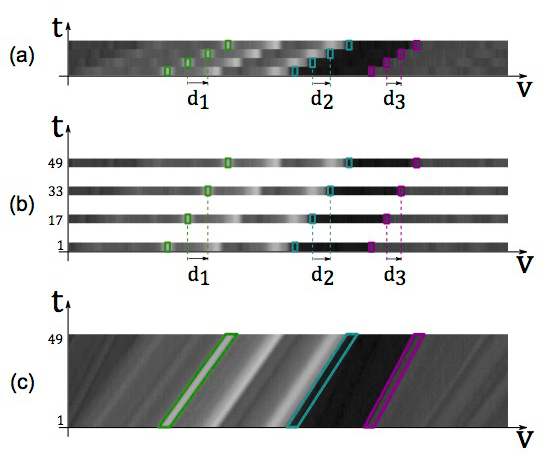
\includegraphics[width=0.6\textwidth]{./Diagrams/sparse_EPI.jpg}
\caption{(a) EPI for a coarsely sampled light field; (b) Correspondeing partially defined densely sampled EPI; (c) Ground truth densely sampled EPI, can be obtaied by inpainting. Figure taken from \cite{LF-Shearlets} pp. 6}
\label{fig:sparse_EPI}
\end{figure}

One would like to recover the lost sections of the EPIs, this task is present in different applications on data processing, since frequently the technologies of data acquisition fails resulting on missing traces; in imaging science, this task is referred as \textit{inpainting} by the similiraty of the physical task of restoring a painting. 

\bigskip

There are different algorithmical approaches to the inpainting task; the algorithms based on variational approaches which propagate information from the boundaries and try to guarantee smoothness (see \cite{Ballester}). Another approach is based on applied harmonic analysis combined with ideas of compressed sensing, assuming that certain representation systems provide sparse approximations of the original image, most of the approaches assume that one knows the position and shape of the lost areas (referred as masks).

\bigskip

In this thesis we will follow the second approach exploiding the sparse representation characteristics of the shearlet systems to inpaint epipolar plane images obtained from a sparsely sampled light field; using a combination of harmonic analysis and also a $\ell^1$ minimization technique widely used in compressed sensing. 

\bigskip

Before explaining the particular case of inpainting algorithm that we will work with it is worthwhile to present a general abstract framework of inpainting to grow some intuition. For this we need a separable Hilbert space $\mathcal{H}$. Let $x^0\in\mathcal{H}$ the undamaged (original) \textit{signal} that we want to recover. We will also assume that $\mathcal{H}$ decomposes into an orthogonal sum of two closed subspaces, that we will call the \textit{known part} and the \textit{missing part}, 

$$
\mathcal{H}=\mathcal{H}_K\oplus\mathcal{H}_M=P_K\mathcal{H}\oplus P_M\mathcal{H}
$$

where $P_K$ and $P_M$ are the orthogonal projection operator to the respective space. The inpainting of $x^0$ will be then translated to: "Given a corrupt signal $P_Kx^0$, recover the missing part $P_Mx^0$. 

\bigskip

In the case of image inpainting, we will consider a continuous image model, where $\mathcal{H}=L^2(\mathbb{R}^2)$, where the missing space is $H_M=L^2(\mathcal{M})$ for some measurable set $\mathcal{M}\subset\mathbb{R}^2$, seen as a mask covering the corrupted parts of the painting. In the next we will make further assumptions on the signal and missing space.

\bigskip

We will assume that the signal $x^0$ can be efficiently represented by some Parseval frame $\Phi=(\phi_i)_{i\in I}$ for $\mathcal{H}$, at practical applications this assumption is reasonable since we already mentioned that natural images represented by cartoon-like functions are optimally represented by directional systems as shearlets or curvelets. In the classical theory of sparse representations, this is translated as asking for the solution of the $\ell^0$-minimization problem

\begin{equation}
\label{eq:alpha21}
\underset{c\in\ell^2(I)}{\min}||c||_{\ell^0(I)}\quad\textrm{subject to}\quad x^0=T_{\Phi}^*c=\sum_{i\in I}c_i\phi_i
\end{equation}

where the operator $T^*_{\Phi}$ is the so-called synthesis operator associated to the frame, then equation~\ref{eq:alpha21} tries to find a synthesis sequence of $x^0$ that has as few as possible non-zero elements measured by $||c||_0:=\#\{c_i|c_i\neq 0\}$, by using the least possible of Shearlet Coefficients one smooth out the masked image covering then the holes get smoothly covered. This minimization problem is not convex which represents a big complexity issue in the solution method; we will then follow a new strategy called \textit{analysis approach}.

\bigskip

In the \textit{analysis approach} we will consider \textit{analysis coefficients} given by the \textit{analysis operator} $T_{\Phi}x^0=(\langle x^0,\phi_i\rangle)_{i\in I}$, since the frame is assumed to obey the Parseval property, we can perform the reconstruction by $x^0=T^*_{\Phi}(\langle x^0,\phi_i\rangle)_{i\in I}=\sum_{i\in I}\langle x^0,\phi\rangle\phi_i$. $\Phi$ is not necessarily a basis, $T_{\Phi}x^0$ might not be a solution of~\ref{eq:alpha21}, so is not yet clear what does it mean to give a sparse representation in the sense of the analysis approach; to make sense of this we need to use some ideas of \textit{compressed sensing}.

\bigskip

To be able to use the \textit{analysis approach} we will introduce the next $\ell^1$-minimization algorithm:

\bigskip

\begin{algorithm}[h!]
    \SetKwInOut{Input}{Input}
    \SetKwInOut{Output}{Output}
		\SetKwInOut{Compute}{Compute}

    \Input{Corrupted signal $P_Kx^0\in\mathcal{H}_K$, Parseval frame $\Phi=(\phi_i)_{i\in I}$ for $\mathcal{H}$}
		\Compute{\begin{equation}
			x^*=\underset{x\in\mathcal{H}}{\text{argmin}}||T_{\Phi}x||_{\ell^1(I)} \quad\textrm{subject to}\quad P_Kx^0=P_Kx
			\tag{$\ell^1-\text{INP}$}
		\label{eq:alphal1}
		\end{equation}}
    \Output{recovered signal $x^*\in\mathcal{H}$}
    \caption{Inpainting via $\ell^1$-minimization}
		\label{alg:alpha21}
\end{algorithm}

\bigskip

In other words, Algorithm~\ref{alg:alpha21} minimizes the $\ell^1$-norm among all possible reconstruction candidates, which is the set of all signals coinciding with $x^0$ on $\mathcal{H}_K$. In the case where the undamaged signal $x^0$ is sufficiently sparsified by $\Phi$, and then it has a small $\ell^1$-norm of $T_{\Phi}x^0$, the solution $x^*$ will provide a good reconstruction of the important features on $x^0$.

\bigskip

We would like to prove some error estimates for the recovery by Algorithm~\ref{alg:alpha21}, for this, we will introduce some analysis tools that will also give us further insight about the structure of the proposed abstract model.

\bigskip

\begin{defn}[$\delta$-cluster sparsity]
\label{def:alpha22}
Let $\delta>0$ and $\Gamma\subset I$. A signal $x\in\mathcal{H}$ is called $\delta$-clustered sparse in $\Phi$ with respect to $\Gamma$, if
\begin{equation}
\label{eq:alpha22}
||\mathbf{1}_{\Gamma^c}T_{\Phi}x||_{\ell^1}\leq \delta
\end{equation}
In this case, $\Gamma$ is said to be $\delta$-cluster for $x$ in $\Phi$. 
\end{defn}

\bigskip

A signal will be $\delta$-clustered sparse if the analysis coefficients are highly concentrated on $\Gamma$. This definition will only have a useful meaning when $x$ is $\delta$-clustered sparse with respect to a small cluster $\Gamma$, and $\delta$ sufficiently small at the same time. Independently we can define the concept of \textit{cluster coherence}.

\bigskip

\begin{defn}[Cluster coherence]
Let $\Gamma\subset I$, the cluster coherence of $\Phi$ with respect to $\mathcal{H}_M$ and $\Gamma$ is given by 
$$
\mu_c(\Gamma,P_M\Phi):=\max_{j\in I}\sum_{i\in\Gamma}|\langle P_M\phi_i,P_M\phi_j\rangle|,
$$
where $P_M\Phi:=(P_M\phi_i)_{i\in I}$.
\end{defn}

\bigskip

The cluster coherence can be understood as an abstract measure for the gap size; we do not know $P_Mx^0$, so we would like to know the maximal amount of missing information. The Parseval expansion $x^0=\sum_{j\in I}\langle x^0,\phi_j\rangle \phi_j$ help us to estimate the analysis coefficientes of its projection onto $\mathcal{H}_M$:

\begin{equation}
\label{eq:alpha23}
|\langle P_Mx^0,\phi_i\rangle|\leq\sum_{i\in I}|\langle x^0,\phi_j\rangle||\langle P_M\phi_j,\phi_i\rangle|=\sum_{i\in I}|\langle x^0,\phi_j\rangle||\langle P_M\phi_j, P_M\phi_i\rangle|.
\end{equation}

The scalar products $|\langle P_M\phi_j,P_M\phi_i\rangle|$ broadly indicate how "correlated" the measurments with $\phi_i$ and $\phi_j$ are on $\mathcal{H}_M$. To compute the recovery error, it was proposed before (see \cite{Firstinpaint}) to estimate the ditance between $x^0$ and its $\ell^1$-recovery $x^*$ with the Hilbert norm. This worked well to estimate an upper bound, but to show an optimality result (lower bound), measuring $||\cdot||$ is not useful, since the Parseval property of $\Phi$ gives $||x^0-x^*||=||T_{\Phi}(x^0-x^*)||_{\ell^2}$, the $\ell^2$-norm in comparison with the $\ell^1$ has an averaging effect on the coefficientes, then some sparsity features might be hidden when using the Hilbert space norm. We will proposed a new norm to measure the error, the $\ell^1$-analysis norm.

\bigskip

\begin{defn}[$\ell^1$-analysis norm]
Let $x\in\mathcal{H}$ and $\Phi$ be a Parseval frame for $\mathcal{H}$. Then we define the $\ell^1$-analysis norm, with respect to $\Phi$, by
$$
||x||_{1,\Phi}:=||T_{\Phi}x||_{\ell^1}=||(\langle x,\phi_i\rangle)_{i\in I}||_{\ell^1}
$$
and the $\ell^1$-analysis space given by 
$$
\mathcal{H}_{1,\Phi}:=\{x\in \mathcal{H}:||x||_{1,\Phi}<\infty\}
$$
equipped with $||\cdot||_{1,\Phi}$
\end{defn}

Since $\Phi$ forms a Parseval frame, its analysis operator $T_{\Phi}$ is injective, and therefore the tuple $(\mathcal{H}_{1,\Phi},||\cdot||_{1,\Phi})$ defines a normed vector space, moreover
\begin{equation}
\label{eq:alpha24}
||x||=||T_{\Phi}x||_{\ell^2}\leq ||T_{\Phi}x||_{\ell^1}=||x||_{1,\Phi}
\end{equation}
then we have the embedding $\mathcal{H}_{1,\Phi}\hookrightarrow\mathcal{H}$, then, by picking $x=x^*-x^0$, we can conclude that small recovery errors in $\mathcal{H}_{1,\Phi}$ always imply small ones in $\mathcal{H}$. With this tools we can provide a estimate of the recovery error.

\begin{thm}
\label{thm:alpha25}
Let $\delta>0$ and $\Gamma\subset I$ be a $\delta$-cluster for $x^0$ in $\Phi$. Moreover, assume that $\mu_c(\Gamma,P_M\Phi)<1/2$. If $x^0\in\mathcal{H}_{1,\Phi}$ then the $\ell^1$-minimizer $x^*$ of the Algorithm~\ref{alg:alpha21} is also contained in $\mathcal{H}_{1,\Phi}$ and satisfies 
\begin{equation}
\label{eq:alpha25}
||x^*-x^0||_{1,\Phi}\leq \frac{2\delta}{1-2\mu_c(\Gamma,P_M\Phi)}
\end{equation}
\end{thm}
\begin{proof}
The proof can be found in \cite{Firstinpaint}.
\end{proof}

\bigskip

The Theorem~\ref{thm:alpha25} gives good estimates if $\Phi$ sparsifies $x^0$ and the size of the missing space, the latter measured in terms of cluster coherence is not too large. We would like to pick a cluster $\Gamma$ such that $x^0$ becomes $\delta$-clustered sparse for small $\delta$ and at the same time $\mu_c$ shall not exceed the bound of $1/2$; even the concepts if cluster sparsity and cluster coherence were introduced independently, both notions are now joined together in terms of $\Gamma$; enlarging $\Gamma$ makes the Equation~\ref{eq:alpha25} true for smalle $\delta$, while $\mu_c(\Gamma,P_M\Phi)$ increases and could exceed $1/2$, this tell us that applying the Theorem~\ref{thm:alpha25} involves actually the fundamental task of choosing an appropriate cluster (see \cite{Firstinpaint} for a more detailed analysis). 

\bigskip

So far we have a general abstract framework for inpainting for Parseval frames, we would like to have an appropriate parseval frame to inpaint natural images (in the case of this thesis Epipolar Plane Images), in the sense that the recovery error is small; we have different options, for instance Universal Shearlet Systems and Wavelet Systems. Theorem~\ref{thm:alpha34} we know that for a scaling sequence $(\alpha_j)_j$ the related Universal Shearlet System $\mathcal{SH}(\phi,v,(\alpha_j)_j)$ form a Parseval frame for $L^2(\mathbb{R}^2)$ and that they behave asymptotically equally as the $\alpha$-Shearlets system $\mathcal{SH}(\phi,\psi,\tilde{\psi};\alpha)$, then the $\alpha$-Shearlets and the Universal Shearlet Transform can be used in the inpainting framework. In the case of the Wavelet Systems, they will also form a frame for $L^2(\mathbb{R}^2)$ under some assumptions on the mother wavelet function, the scaling and the translation parameter (see \cite{Mallat} pp. 202).

\bigskip

In order to compare the shearlets and the wavelets performance for inpaiting, we want to present a benchmark that is related to the principal problem of the thesis, that is the inpainting of sparse sampled epipolar plane images (see Figure~\ref{fig:sparse_EPI}). Cartoon-like images are we know are governed by edges, the image to be inpainted as a benchmark is a masked linear singularity that can be viewed as a strip; epipolar plane images corresponding to sparse sampled light fields have also strips as missing space so this example will be enough. Many details in the analysis will be ommited but they are well explained in \cite{Gitta-alpha}. 

\bigskip

As we cannot work on actual edges in $L^2(\mathbb{R}^2)$ and other Lebesgue spaces since they have measure zero, we will work with a line-distribution given by $\omega\mathcal{L}$ acting on Schwartz functions $f\in\mathbb{S}(\mathbb{R}^2)$, i.e.\ $\omega\mathcal{L}\in \mathbb{S}'(\mathbb{R}^2)$, if $\text{supp }\omega\subset[-\rho,\rho]$ then its action will be defined by

$$
\langle \omega \mathcal{L},g\rangle = \int_{-\rho}^{\rho} \omega(x_1)g(x_1,0)dx_1 \textrm{,}\quad \forall g\in\mathcal{S}(\mathbb{R}^2)
$$

where $\omega$ is a smooth weight and $\rho>0$. The weight $\omega$ sets up the linear singularity that is smooth in the vertical direction, while the value of $\rho$ corresponds to the length of the singularity. We will mask the linear singularity (weighted distribution) $\omega\mathcal{L}$ with the mask 

$$
M_h=\{(x_1,x_2)\in\mathbb{R}^2:|x_1|\leq h\}\textrm{,}\quad h>0
$$

The observed signal then is 
$$
f=\mathbf{1}_{\mathbb{R}^2\setminus M_h}\cdot \omega\mathcal{L}
$$ 

see Figure~\ref{fig:alpha6}. We decompose $\omega\mathcal{L}$ by the same subbands $F_j$, $\omega\mathcal{L}\mapsto \omega\mathcal{L}_j=\omega\mathcal{L}*F_j$, denote $h=h_j$ and set 

$$
f_j=\mathbf{1}_{\mathbb{R}^2\setminus M_{h_j}}\cdot \omega\mathcal{L}_j
$$

\begin{figure}[h!]
\centering
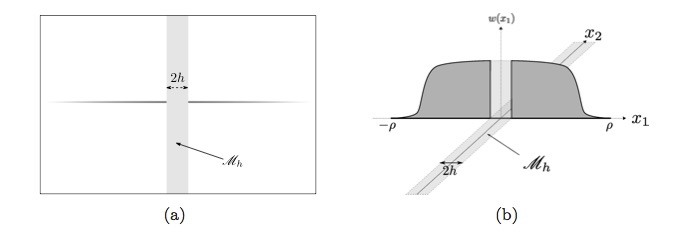
\includegraphics[width = 0.9 \textwidth]{./Diagrams/alpha6.jpg}
\caption{(a) Sketch of the corrupted modeling image, the line singularity has no "thickness" but some (gray-scale) intensity. (b) "Graph" of the corrupted line distribution $P_K\omega\mathcal{L}$ which is compactly supported on the $x_1$-axis. Figure taken from \cite{Gitta-alpha} pp. 15}
\label{fig:alpha6}
\end{figure}

\bigskip

Let $\{\psi_{\lambda}\}$ denote a particular wavelet Parseval frame and $\{ \sigma_{\eta}\}_{\eta}$ a particular shearlet Parseval frame (could be, classical shearlets, cone-adapted shearlets, $\alpha$-shearlets or universal shearlets). Then we can rewrite the minimization problem~\ref{eq:alphal1} as

$$
W_j=\underset{\tilde{W}_j}{\textrm{argmin}}||(\langle \tilde{W}_j,\psi_{\lambda}\rangle )_{\lambda}||_{\ell^1}\quad\textrm{subject to}\quad f_j=\mathbf{1}_{\mathbb{R}^2\setminus M_{h_j}}\cdot\tilde{W}_j
$$ 

for wavelet-based inpainting and 

$$
S_j=\underset{\tilde{S}_j}{\textrm{argmin}}||(\langle \tilde{S}_j,\sigma_{\eta}\rangle)_{\eta}||_{\ell^1}\quad \textrm{subject to}\quad f_j=\mathbf{1}_{\mathcal{R}^2\setminus M_{h_j}}\cdot\tilde{S}_j
$$

for the shearlet-based inpainting. Now we can state a Theorem that compares both systems in the inpainting task.

\begin{thm}
\label{thm:inpaintingwaveletsshearlets}
For $h_j=o(2^{-j})$ (the critical thresholding case) as $j\longrightarrow \infty$,
$$
\frac{||W_j-\omega\mathcal{L}_j||_2}{||\omega\mathcal{L}_j||_2}\longrightarrow 0\textrm{,}\quad j\longrightarrow \infty\\
$$ 
For $h_j=o(2^{-j/2})$ as $j\longrightarrow\infty$,
$$
\frac{||S_j-\omega\mathcal{L}_k||_2}{||\omega\mathcal{L}_j||_2}\longrightarrow 0\textrm{,}\quad j\longrightarrow\infty\\
$$
\end{thm}
\begin{proof}
Due the technical level of the proof, we will refer to \cite{clustered-inpainting} for the detailed proof. 
\end{proof}

The Theorem~\ref{thm:inpaintingwaveletsshearlets} shows that Shearlets is a better choice than Wavelets as a Sparsifying  Parseval Frame to perform the inpainting of natural images, in particular of EPIs, therefore is the system that we picked in this thesis.

\bigskip

There are different methods to minimize the $\ell^1$-norm in the inpainting algorithm~\ref{alg:alpha21}, we will use the iterative hard thresholding method since is the one that is traditionally used due to its effectiveness, the implementation and application of this algorithm for our task of EPIs-inpatinting will be explained in the Chapter~\ref{chap:Inpainting_sparse}.

\section{0-Shearlets}
\label{sec:0-Shearlets}

In the last section we introduce a generalization of the classical cone-adpated shearlet transform allowing a more flexible scaling matrix $A_{j,\alpha_j,(\iota)}$, where $\alpha_j\in (-\infty,2)$ changes the "level" of anisotropy of the features the transform is sensible to. We also know by Theorem~\ref{thm:alpha34} that Shearlet System generated by the sequence of scaling parameters $(\alpha_j)_{j\in\mathbb{N}_0}$ will form a frame if the sequence form a scaling sequence, i.e.\ $\alpha_j$ is a multiple of $2/j$.

\bigskip

 In the case when $\alpha_j=2$ for all $j=2$ we have a isotropic scaling case, where isotropic features like circles are well represented; it is the case of the wavelets. In the other hand when $\alpha_j=1$ for all $j$, then we have the classical cone-adapted shearlet system and the related parabolic scaling is well suited to approximate functions with singularities over parabolic curves. 

\bigskip

As we already mentioned several times, the final task of this thesis is to inpaint EPIs form sparse sampled light fields using Shearlets. As we can see in Figure~\ref{fig:sparse_EPI} Epipolar Plane Images consist of straight-line structures, so one would like to have a scaling operation suited to straight-lines; this is performed using the sequence of scaling parameters given by

$$
\alpha_j=-\frac{2}{j}\in A_j\textrm{,}\quad \forall j\in\mathbb{Z}
$$

therefore the related universal shearlet system will form a Parseval frame and our inpainting framework is valid. By choosing like in this case very small $\alpha_j$ one produces more anisotropic elements which will approximate properly straight-line formed structures.

\bigskip

As we saw in Section~\ref{sec:shearletsystem}, the generating functions of a cone-adapted separable compactly supported shearlet system are given by:

$$
\begin{aligned}
\psi(x_1,x_2)&=\psi_1(x_1)\phi_1(x_2)\\
\phi(x_1,x_2)&=\phi_1(x_1)\phi_1(x_2)\\
\tilde{\psi}(x_1,x_2)&=\psi(x_2,x_1)
\end{aligned}
$$

where $\phi_1$ and $\psi_1$ are 1D scaling and wavelet functions. To obtain a smaller overlaping of the elements in the fourier transform one can multiply the separable generator by a 2D directional fan filter
$$
\hat{\psi}^{\text{nonsep}}=P(\xi_1/2,\xi_2)\hat{\psi}_1(\xi_1)\hat{\phi}_1(\xi_2)
$$ 

\bigskip

If one considers a multiresolution analysis with wavelet and scaling function $\psi_1,\phi_1\in L^2(\mathbb{R}^2)$ given by
$$
\begin{aligned}
\phi_1(x_1)&=\sum_{n_1\in\mathbb{Z}}h(n_1)\sqrt{2}\phi_1(2x_1-n_1)\\
\psi_1(x_1)&=\sum_{n_1\in\mathbb{Z}}g(n_1)\sqrt{2}\phi_1(2x_1-n_1)
\end{aligned}
$$

\bigskip

The universal shearlet system generated by the scaling sequence $(\alpha_j)_{j\in \mathbb{Z}}=(-2/j)_{j\in\mathbb{Z}}$ will be referred as $0-Shearlets$ since $\alpha_j\underset{j\rightarrow\infty}\longrightarrow 0$. The scaling matrix related to the $0$-shearlets will be given by
$$
A_{j}=\left(\begin{matrix} 2^j & 0\\ 0 & 2^{-1}\end{matrix}\right)
$$

The choice as expected will provide scaling only by one axis and the shearing will change the direction of the scaling. Let $J\in\mathbb{N}$ the maximum scale, then the shearlet system for $\Psi(\psi)$ is formed by the functions

$$
\Psi(c,\psi)=\psi_{j,k,m}\textrm{,}\quad |k|\leq 2^{j+1}\textrm{,}\quad j=0,\ldots,J-1,
$$

where

\begin{equation}
\label{eq:LFshearlets3}
\psi_{j,k,m}(x)=2^{j/2}\psi(S_kA_jx-M_{c_j}m),
\end{equation}

and $c_j=(c_1^j,c_2^j)$ are sampling constants for translation. It is easy to see that

\begin{equation}
\label{eq:LFshearlets4}
\psi_{j,k,m}(x)=\psi_{j,0,m}\left( S_{\frac{k}{2^j+1}}x\right).
\end{equation}

Following the procedure of \cite{Shearlab}, it can be shown that the digital filter corresponding to $\psi_{j,0,m}$ is given by

\begin{equation}
\label{eq:LFshearlets5}
\psi^d_{j,0}(m)=(p_j\ast(g_{J-j}\otimes h_{J+1}))(m),
\end{equation}

where $\otimes$ denote the tensor product such that 

$$
(g_{J-j}\otimes h_{J+1})(m)=g_{J-j}(m_1)h_{J+1}(m_2),
$$

and $\{p_j(n)\}_{n\in\mathbb{Z}}$ are the Fourier coefficients of the trigonometric polynomial $P(2^{J-j-1}\xi_1,2^{J+1}\xi_1)$, $\{ h_j(n)\}_{n\in\mathbb{Z}}$ and $\{g_j(n)\}_{n\in\mathbb{Z}}$ are the Fourier coefficients of the respective trigonometric polynomial

$$
\begin{aligned}
\hat{h}_j(\xi)&=\prod_{k=0,\ldots,j-1}\hat{h}(2^k\xi),\\
\hat{g}_j(\xi)&=\hat{g}(2^{j-1}\xi)\hat{h}_{j-1}(\xi)
\end{aligned}
$$

and $\hat{h}_0\equiv 1$, one can see in Figure~\ref{fig:magnitude_response} the frequency responses of this digital filters until scale $j=4$. 

\begin{figure}[h!]
\centering
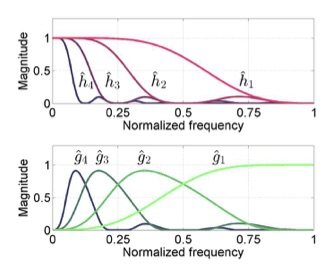
\includegraphics[width = 0.7 \textwidth]{./Diagrams/magnitude_response.jpg}
\caption{Frequency responses of the scaling and wavelet filters $h_j,g_j,j=1,\ldots,4$. Figure taken from \cite{LF-Shearlets} pp. 4}
\label{fig:magnitude_response}
\end{figure}

As it was presented for first time in \cite{Nonseparableshear}, the shearing transform $S_{k2^{-j}}$, $j\in\mathbb{N}$, $k\in\mathbb{Z}$ does not preserve the regular grit $\mathbb{Z}^2$, therefore its digitalization is non-trivial. To tackle this issue, one needs to refine the $\mathbb{Z}^2$ grid along the $x_1-axis$ by a factor $2^j$, then the new grid $2^{-j}\mathbb{Z}\times\mathbb{Z}$ is invariant under the $S_{k 2^{-j}}$ transform. 

\bigskip

For an arbitrary $r\in \ell^2(\mathbb{Z}^2)$, the shear transform $S_{k 2^{-j}}$ can be implemented as a digital filter

\begin{equation}
\label{eq:LFshearlets6}
S^d_{k 2^{-j}}(r)=((2^jr_{\uparrow 2^j}\ast_1\tau_j)(S_k\cdot)\ast_1\overline{\tau}_j)_{\downarrow 2^j}
\end{equation}

where $\tau_j$ is a digital low-pass filter with normalized cutoff frequency at $2^{-j}$. 

\bigskip

Using the Equations~\ref{eq:LFshearlets3},~\ref{eq:LFshearlets4},~\ref{eq:LFshearlets5} and~\ref{eq:LFshearlets6} and the proper choice of $c_j$ it can be shown that the digital filter corresponding to $\psi_{j,k,m}$ is given by

$$
\psi_{j,k}^d(m)=(S^d_{k2^{-(j+1)}}(p_j\ast g_{J-j}\otimes h_{J+1}))(m).
$$

A digital filter corresponding to separable elements of the transform $\phi_m$ related to the scaling function, is given by $\phi^d=(h_J\otimes h_J)(m)$. Then, the discrete shearlet transform associated with the set of elements $\Psi(c;\psi)$ and corresponding to frequency plane region $C_{\psi}$ is defined as follows

$$
\mathcal{DST}_{j,k,m}(f_J)=(f_J\ast \overline{\psi_{j,k}^d})(m),
$$

where $f_J(n)$ for $n\in\mathbb{Z}^2$ are discrete samples of $f\in L^2(\mathbb{R}^2)$, $j=0,\ldots,J-1$, $|k|\leq 2^{j+1}$, $m\in\mathbb{Z}^2$.

\bigskip

To compute the inverse transform we need to construct the dual frame; in order to do that we first set

$$
\hat{\Psi}^d=|\hat{\phi}^d|^2+\sum_{j=0,\ldots,J-1}\sum_{|k|\leq 2^{j+1}}(|\hat{\psi}^d_{j,k}|^2+|\hat{\tilde{\psi}}_{j,k}^d|^2).
$$ 

The dual shearlet filters are defined by

$$
\hat{\phi}^d=\frac{\hat{\phi}^d}{\hat{\Psi}^d}\textrm{,}\quad \hat{\gamma}^d_{j,k}=\frac{\hat{\psi}^d_{j,k}}{\hat{\Psi}^d}\textrm{,}\quad \hat{\tilde{\gamma}}^d_{j,k}=\frac{\hat{\tilde{\psi}}_{j,k}^d}{\hat{\Psi}^d}
$$

\begin{figure}[h!]
\centering
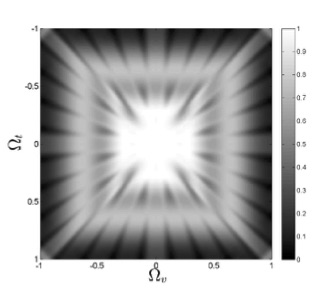
\includegraphics[width = 0.7 \textwidth]{./Diagrams/LFshearlets2e.jpg}
\caption{$\hat{\Psi}^d$ corresponding to constructed shearlet transform for $J=2$. Figure taken from \cite{LF-Shearlets} pp. 4}
\label{fig:LFshearlets2e}
\end{figure}

\begin{figure}[h!]
\centering
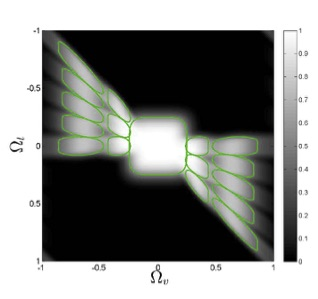
\includegraphics[width = 0.7 \textwidth]{./Diagrams/LFshearlets2f.jpg}
\caption{Frequency domain support of shearlet transform elements used in reconstruction. Figure taken from \cite{LF-Shearlets} pp. 4}
\label{fig:LFshearlets2f}
\end{figure}

One can see an illustration of the obtained system in the frequency plane $\hat{\Psi}^d$ for $J=2$ in Figure~\ref{fig:LFshearlets2e}. Finally, the reconstruction formula is given by

$$
f_J=(f_J\ast \overline{\phi}^d)\ast \phi^d+\sum_{j,k}(f_J\ast\overline{\psi}^d_{j,k})\ast \gamma^d_{j,k}+\sum_{j,k}(f_J\ast \overline{\tilde{\psi}}^d_{j,k})\tilde{\gamma}^d_{j,k}
$$

Following the methodology of \cite{LF-Shearlets} we will be interested only in the transform elements where the shearing has positive sign, i.e. $0\leq k\leq 2^{j+1}$, the corresponding transform elements are ccovering the frequency domain region highlighted in Figure~\ref{fig:LFshearlets2f}. Then, we use the direct transform $S$ for discrete values $f_J$ and $j=0,\ldots J-1$, $k=0,\ldots, 2^{j+1}$, $m\in\mathbb{Z}^2$ defined as 

\begin{equation}
\label{eq:0analysis}
S(f_J)=\{ c_{j,k}(m)=(f_J\ast \overline{\psi}_{j,k}^d)(m),c_0(m)=(f_J\ast \overline{\phi}^d)(m):\quad j=0,\ldots,J-1,k\leq 2^{j+1},m\in\mathbb{Z}^2\}.
\end{equation}

where $S$ is known as the synthesis operator related to the $0$-Shearlets frame. The inverse transform $S^*$ is then given by the so called synthesis operator 

\begin{equation}
\label{eq:0synthesis}
S^*(\{c_{j,k},c_0\})=\sum_{\begin{matrix}j=0,\ldots,J-1\\k=0,\ldots,2^{j+1}\end{matrix}}(c\ast \gamma_{j,k}^d)(m)+(c_0\ast\phi^d)(m).
\end{equation}

In the case of the Shearlet Transform implementation that we used for this thesis (Shearlab.jl) the $0$-Shearlet transform can be perform by choosing for each scale $j$ the number of shearings to be such that $|k|\leq 2^{j+1}$.

\bigskip

As a final remark for this section it is worth to mention that the $0$-Shearlet system is closely related to the Ridgelet Transform (see \cite{ridglet}), in the sense that both are computed by an inner product of an admissible generating function with different directional, scaling and translational parameters, where the scaling operation is performed in just one direction; the difference is that ridgelets perform directional operation by rotating the elements instead of shearing.

\bigskip

We have now all the tools necessary to perform the light field reconstruction using the Epipolar Plane Images method with sparsely sampled EPIs; in the next chapter we will present the minimization method used to perform such reconstruction as well as the results obtained numerically and the comparison with other light field reconstruction methods using different softwares and procedures. 
